
\pdfminorversion=7
\documentclass[
    sigconf,                        % conference layout
    nonacm,                         % do not include ACM headers/footers
    balance=false,                  % for balancing the last page
    natbib=false,                   % we use BibLaTex & Biber
    pdfa,                           % PDF/A conformance in hyperref
    svgnames,                       % load xcolor with more named colors
]{acmart}

%%%%%%% Packages %%%%%%%
\usepackage[
    linesnumbered,
    norelsize,
    ruled,
    vlined
]{algorithm2e}                      % pseudo code
\usepackage[
    datamodel=acmdatamodel,
    style=acmnumeric,
    backend=biber,
]{biblatex}                         % BibLaTex with custom ACM style
\usepackage{enumitem}               % for customizing bullet points
\usepackage{etoolbox}               % command patching
\usepackage{flushend}               % balanced columns on last page
\usepackage[edges]{forest}          % drawing flow charts
\usepackage{hyphenat}               % hyphenation for words with hyphens
\usepackage{mathtools}              % math notation
\usepackage{subcaption}             % subfigures/subtables
\usepackage{tabularx}               % variable length table columns
\usepackage[
    skins,
    breakable
]{tcolorbox}                        % for colored text boxes
\usepackage{tikz}                   % drawings

% These packages are used but already recursively loaded by other packages
\usepackage{booktabs}               % professional tables
\usepackage{graphicx}               % figures
\usepackage{microtype}              % better typography

%%%%%%% Bibliography %%%%%%%
% General Options
\ExecuteBibliographyOptions{
    block=space,
    minbibnames=3,
    maxbibnames=4,
    maxcitenames=2,
    % giveninits=true,
    date=year,
    doi=false,
    eprint=false,
    isbn=false,
    url=false,
}
\ExecuteBibliographyOptions[software]{
    url=true
}
\ExecuteBibliographyOptions[report]{
    url=true
}
\setcounter{biburllcpenalty}{7000}

% Item formatting
\AtEveryBibitem{
    \clearfield{day}
    \clearfield{note}
    \clearfield{month}
    % \clearfield{pages}
    \clearfield{pagetotal}
    \ifentrytype{inproceedings}{
        % \clearfield{booktitle}
        \clearfield{eventtitle}
        % \clearfield{pages}
        % \clearfield{series}
        \clearfield{volume}
        \clearlist{location}
        \clearlist{publisher}
        \clearname{editor}
    }{}
    \ifentrytype{article}{
        % \clearfield{number}
        % \clearfield{pages}
        % \clearfield{volume}
    }{}
    \ifentrytype{incollection}{
        \clearfield{volume}
        \clearlist{location}
        % \clearlist{publisher}
        % \clearname{editor}
        \clearfield{edition}
    }{}
    \ifentrytype{book}{
        \clearlist{location}
    }{}
    \ifentrytype{software}{
        \clearfield{urlyear}
    }{}
}
% \renewbibmacro{in:}{\ifentrytype{inproceedings}{}{\printtext{\bibstring{in} }}}
\renewbibmacro{in:}{\ifentrytype{inproceedings}{}{\printtext{\bibstring{in}\intitlepunct}}}
\DeclareFieldFormat[inproceedings]{booktitle}{\mkbibemph{Proceedings of the #1}}
\DeclareFieldFormat{series}{\mkbibemph{#1}}
\DeclareFieldFormat{titlecase}{#1}

% \DeclareSourcemap{
%     \maps[datatype=bibtex]{
%         \map{
%             \pertype{inproceedings}
%             \step[fieldsource=eventtitle, match=\regexp{(.*)....$}, replace=\regexp{$1}]
%         }
%     }
% }

% Hyphenation overwrites
\hyphenation{Mah-di-ra-ji}

% Reference font size
\renewcommand*{\bibfont}{\normalfont\small}

% Bib files
\addbibresource{bib/references.bib}


%%%%%%% Custom Commands %%%%%%%
\newcommand{\system}[0]{\textsc{Fain\-der}}
\newcommand{\exact}[0]{\textsc{Fain\-der Exact}}
\newcommand{\approximate}[0]{\textsc{Fain\-der Approx}}
\newcommand{\pscan}{\texttt{pro\-file\hyp{}scan}\xspace}
\newcommand{\binsort}{\texttt{binsort}\xspace}
\newcommand{\ndist}{\texttt{nor\-mal\hyp{}dist}\xspace}
\newcommand{\edges}[1]{\FuncSty{edges} (#1)}
\newcommand{\density}[1]{\FuncSty{density} (#1)}

\newcommand\cA{\mathcal{A}}
\newcommand\cB{\mathcal{B}}
\newcommand\cD{\mathcal{D}}
\newcommand\cH{\mathcal{H}}
\newcommand\cI{\mathcal{I}}
\newcommand\cK{\mathcal{K}}
\newcommand\cM{\mathcal{M}}
\newcommand\cP{\mathcal{P}}
\newcommand\cS{\mathcal{S}}

\newcommand{\sset}[1]{\left\{\,#1\,\right\}} % { ? }, automatic brackets
\newcommand\bR{\mathbb{R}} % set of reals
\newcommand\true{\text{true}} % Booleans in math mode
\newcommand\false{\text{false}} % Booleans in math mode

%%%%%%% Layout settings %%%%%%%
% ACM template changes
\settopmatter{authorsperrow=4}
\makeatletter
\renewcommand\paragraph{\@startsection{paragraph}{4}{0\p@}%
{-.1\baselineskip \@plus -2\p@ \@minus -.2\p@}%
{-3.5\p@}%
{\ACM@NRadjust{\bfseries\@adddotafter}}}
\makeatother

% Algorithm2e
\SetAlFnt{\footnotesize}
\DontPrintSemicolon
\let\oldnl\nl% Store \nl in \oldnl
\newcommand{\nonl}{\renewcommand{\nl}{\let\nl\oldnl}}% Remove line number for one line
\newcommand\commentstyle[1]{\scriptsize\ttfamily\textcolor{gray}{#1}}
\SetCommentSty{commentstyle}
\makeatletter
% Remove right hand margin in algorithm
\patchcmd{\@algocf@start}% <cmd>
{-1.5em}% <search>
{0pt}% <replace>
{}{}% <success><failure>
\makeatother

% Tikz and math
\usetikzlibrary{arrows, arrows.meta, backgrounds, calc, fit, matrix, patterns, positioning, shapes, shapes.arrows, shapes.misc, trees}

\pgfdeclarelayer{foreground}
\pgfdeclarelayer{background}
\pgfsetlayers{background,main,foreground}

\newcommand*{\circled}[1]{%
    \tikz[baseline=(char.base)]{\node[shape=circle,draw,inner sep=0.5pt, fill=lightgray] (char) {\small #1};}%
}

\tikzset{bound/.style={draw,dashed,gray,rounded corners}}
\tikzset{fit margins/.style={/tikz/afit/.cd,#1,
    /tikz/.cd,
    inner xsep=\pgfkeysvalueof{/tikz/afit/left}+\pgfkeysvalueof{/tikz/afit/right},
    inner ysep=\pgfkeysvalueof{/tikz/afit/top}+\pgfkeysvalueof{/tikz/afit/bottom},
    xshift=-\pgfkeysvalueof{/tikz/afit/left}+\pgfkeysvalueof{/tikz/afit/right},
    yshift=-\pgfkeysvalueof{/tikz/afit/bottom}+\pgfkeysvalueof{/tikz/afit/top}},
    afit/.cd,left/.initial=2pt,right/.initial=2pt,bottom/.initial=2pt,top/.initial=2pt}

\thinmuskip=0mu plus 2mu minus 1mu
\medmuskip=1mu plus 3mu minus 1mu
\thickmuskip=2mu plus 4mu minus 1mu

\newtheoremstyle{custom}% 〈name〉
    {0.3\baselineskip plus 2pt minus 2pt}% 〈Space above>
    {0.3\baselineskip plus 2pt minus 2pt}% 〈Space below>
    {\itshape}% 〈Body font>
    {\parindent}% 〈Indent amount>
    {\scshape}% 〈Theorem head font
    {.}% 〈Punctuation after theorem head
    {3.5pt}% 〈Space after theorem head>
    {}% 〈Theorem head spec (can be left empty, meaning ‘normal’ )
\theoremstyle{custom}
\newtheorem*{definition}{Definition}
\newtheorem*{example}{Example}
\newtheorem*{problem}{Problem}

% Floats
\setlength{\floatsep}{6pt plus 1pt minus 2pt}{}
\setlength{\textfloatsep}{5pt plus 0pt minus 2pt}
\setlength{\intextsep}{6pt plus 1pt minus 2pt}
\captionsetup[figure]{belowskip=0.0em, aboveskip=0.25em}
\captionsetup[subfigure]{belowskip=0.0em, aboveskip=0.25em}
\captionsetup[table]{belowskip=0.0em, aboveskip=0.25em}

\newlength{\oldcolumnsep}
\setlength{\oldcolumnsep}{\columnsep}

%%%%%%% VLDB settings %%%%%%%
%% The following content must be adapted for the final version
% paper-specific
\newcommand\vldbdoi{10.14778/3681954.3681999}
\newcommand\vldbpages{3269 - 3282}
% issue-specific
\newcommand\vldbvolume{17}
\newcommand\vldbissue{11}
\newcommand\vldbyear{2024}
% should be fine as it is
\newcommand\vldbauthors{\authors}
\newcommand\vldbtitle{\shorttitle}
% leave empty if no availability url should be set
\newcommand\vldbavailabilityurl{https://github.com/lbhm/fainder}
% whether page numbers should be shown or not, use 'plain' for review versions, 'empty' for camera-ready
\newcommand\vldbpagestyle{empty}

%%%%%%% Authors & Title %%%%%%%
\author{Lennart Behme}
\affiliation{%
    \institution{BIFOLD \& TU Berlin}
    \city{}
    \country{}
}
\email{l.behme@tu-berlin.de}

\author{Sainyam Galhotra}
\affiliation{%
    \institution{Cornell University}
    \city{}
    \country{}
}
\email{sg@cs.cornell.edu}

\author{Kaustubh Beedkar}
\affiliation{%
    \institution{IIT Delhi}
    \city{}
    \country{}
}
\email{kbeedkar@cse.iitd.ac.in}

\author{Volker Markl}
\affiliation{%
    \institution{BIFOLD, TU Berlin \& DFKI}
    \city{}
    \country{}
}
\email{volker.markl@tu-berlin.de}

\renewcommand{\shortauthors}{L. Behme et al.}

\title[\system{}: A Fast and Accurate Index for Distribution-Aware Dataset Search]{\system{}: A Fast and Accurate Index\texorpdfstring{\\}{ }for Distribution-Aware Dataset Search}

%%%%%%% Metadata %%%%%%%
\hypersetup{%
    hidelinks,
    bookmarksnumbered,
    unicode,
    pdflang={en},
    pdfstartview=Fit,
    pdfdisplaydoctitle,
    pdfauthor=\vldbauthors,
    pdftitle=\vldbtitle,
    pdfkeywords={data discovery, dataset search},
    pdfapart=2,
    pdfaconformance=B,
}

\begin{document}

%%%%%%% Abstract %%%%%%%
%!TEX root = ../main.tex

\begin{abstract}
Efficient data discovery is crucial in the era of data-driven decision-making.
However, current practices face significant challenges due to the intricacies of identifying datasets with specific distributional characteristics, such as percentiles, when data repositories are decentralized.
Traditional keyword-based search methods are insufficient for these complex requirements, often resulting in suboptimal dataset search results.
To address these challenges, this paper presents \system{}, a fast and accurate index for ``percentile predicates'' on histogram-based data summaries, which streamlines the search process for datasets with specific distributional requirements.
\system{} can be constructed on heterogeneous histogram collections and employs binary search in conjunction with multi-step pruning techniques to efficiently identify search results for percentile predicates.
Thereby, it simplifies data provisioning and improves the effectiveness of dataset discovery.
Empirical evaluation of our solution on three large-scale data repositories shows that \system{} is effective for distribution-aware dataset search and provides order-of-magnitude efficiency gains over baselines.
\end{abstract}


\maketitle

%%% do not modify the following VLDB block %%
%%% VLDB block start %%%
\pagestyle{\vldbpagestyle}
\begingroup\small\noindent\raggedright\textbf{PVLDB Reference Format:}\\
\vldbauthors. \vldbtitle. PVLDB, \vldbvolume(\vldbissue): \vldbpages, \vldbyear.\\
\href{https://doi.org/\vldbdoi}{doi:\vldbdoi}
\endgroup
\begingroup
\renewcommand\thefootnote{}\footnote{\noindent
This work is licensed under the Creative Commons BY-NC-ND 4.0 International License. Visit \url{https://creativecommons.org/licenses/by-nc-nd/4.0/} to view a copy of this license. For any use beyond those covered by this license, obtain permission by emailing \href{mailto:info@vldb.org}{info@vldb.org}. Copyright is held by the owner/author(s). Publication rights licensed to the VLDB Endowment. \\
\raggedright Proceedings of the VLDB Endowment, Vol. \vldbvolume, No. \vldbissue\ %
ISSN 2150-8097. \\
\href{https://doi.org/\vldbdoi}{doi:\vldbdoi} \\
}\addtocounter{footnote}{-1}\endgroup

\ifdefempty{\vldbavailabilityurl}{}{
\vspace{.3cm}
\begingroup\small\noindent\raggedright\textbf{PVLDB Artifact Availability:}\\
The source code, data, and/or other artifacts have been made available at \url{\vldbavailabilityurl}.
\endgroup
}
%%% VLDB block end %%%

%!TEX root = ../main.tex

\section{Introduction}
\label{sec:intro}

In today's data-driven world, where organizations collect vast amounts of information from various sources, efficient and effective data discovery has become indispensable.
The increasing importance of data discovery is primarily driven by the growing popularity of machine learning techniques, which require substantial volumes of data.
Consequently, this trend has led to a surge in data sharing and trading within and across organizations~\cite{azcoitia_survey_2022, kennedy_revisiting_2022}.

However, most data discovery systems (and hence data sharing platforms) have limited utility due to two critical design choices that we summarize in Table~\ref{tab:solution_space}.
First, these systems typically assume that all datasets are \emph{completely accessible to the search algorithm} for indexing and processing~\cite{castelo_auctus_2021, castro_fernandez_aurum_2018, galhotra_metam_2023, gong_ver_2023}.
This assumption neglects the distributed nature of data repositories.
Moving data to a central server is often infeasible due to cost reasons and data owners' reluctance to relinquish control over their proprietary datasets.
Instead, a widely adopted data-sharing paradigm involves a distributed collection of data repositories, where each data provider only shares the \emph{metadata} with a search engine.
This is commonly observed in data market platforms, such as Datarade~\cite{datarade_find_2024} and Dawex~\cite{dawex_data_2024}, as well as federated data settings, such as Gaia-X~\cite{braud_road_2021} and Agora~\cite{traub_agora_2021}.
Second, existing systems generally depend on users conducting keyword search along with filters or providing example data to find relevant datasets~\cite{castelo_auctus_2021, noy_google_2019}.
Even though this search mode is intuitive, it limits discovery in scenarios where users have specific data distribution requirements.
For example, users training a machine learning model might seek datasets with a substantial number of samples from each target group to avoid overfitting.
More broadly, lack of access to a representative sample for data analysis (also known as selection bias) leads to flawed and unreliable outcomes.
These challenges are particularly evident in industrial settings due to repurposing or reusing data~\cite{bethlehem_selection_2010, culotta_reducing_2014, greenacre_importance_2016, zhu_consistent_2023}.
Several data science pipelines have failed because of poor representation of training data~\cite{dastin_amazon_2022, mulshine_major_2015, rose_are_2010, townsend_most_2017}.\looseness=-1

\begin{table}[t]
    \caption{Overview of query-driven dataset search approaches, categorized by search mode and data access model.}
    \label{tab:solution_space}
    \centering
    \begin{tabularx}{\linewidth}{>{\raggedright\arraybackslash}X c c}
        \toprule
        & \multicolumn{2}{c}{Data access model} \\
        \cmidrule{2-3}
        Search mode & Full access & Metadata access\\
        \midrule
        Keyword & \cite{castelo_auctus_2021, castro_fernandez_aurum_2018} & \cite{noy_google_2019, open_knowledge_foundation_ckan_2022, zhang_ad_2018} \\
        By example$^\ddagger$ & \cite{bharadwaj_discovering_2021, bogatu_dataset_2020, castelo_auctus_2021, castro_fernandez_aurum_2018, rezig_dice_2021, santos_sketch-based_2022} & - \\
        Distribution-aware & \cite{asudeh_towards_2022, chai_selective_2022, nargesian_tailoring_2021} & \system{} \\
        \bottomrule
    \end{tabularx}
    \raggedright\footnotesize
    $^\ddagger$ This includes finding joinable and unionable tables based on an input table.\\
\end{table}

Together, the full data access assumption and restricted search mode form a critical roadblock in developing practical data discovery systems.
We demonstrate this with the following example.

\begin{example}
Consider a data scientist training a cancer prediction model.
After developing a prototype, they want to test the robustness of their solution with data from similar trials at other hospitals.
To qualify for their work, a dataset must cover different patient ages, so at least 30\% of patients should be younger than 40 and at least 30\% older than 60.
Since such studies contain sensitive information, accessing them requires approval.
Therefore, the datasets are not centrally gathered but hosted by the organizations that own each dataset.
Consequently, the scientist must search through the publicly available metadata of datasets across several independent data repositories.
\end{example}

While the status quo for search over decentralized data provides basic functionality, it fails to address the nuanced complexities of searching datasets with distributional requirements.
In the example above, our medical scientist only has two options when using keyword-based dataset search: (1)~either pose a general keyword query (e.g.,~``cancer'') and manually review a large number of datasets or (2)~add more keywords to the query, hoping that all those keywords are included in the dataset description so that no relevant dataset is filtered out.
As a consequence of these functional limitations, users often face too many, off-topic, or no results at all.


In this work, we study the novel problem of distribution-aware dataset search over decentralized data repositories, which complements existing search paradigms.
To address the problem, we must tackle three main challenges:
(C1)~We must develop easily adoptable methods for searching over decentralized datasets;
(C2)~users must be able to express distributional requirements in search queries; and
(C3)~search engines must identify datasets that satisfy distributional requirements accurately and efficiently at scale.
To address all these challenges, we propose \system{}, an index for distribution-aware data discovery without raw data access, and a new query model.

\paragraph{(C1) Dataset profiles for search over decentralized data.}
Similar to existing data discovery systems, \system{} assumes that data providers share a profile for each of their datasets with a search engine.
To lower the barrier to enriching existing dataset profiles with distribution-aware data synopses, a solution must require as little additional information and effort beyond the status quo as possible.
One of the most widespread and simple yet flexible synopses are histograms~\cite{cormode_synopses_2011}.
They are easy for data owners to generate and seamlessly integrate into dataset profiles.
Some dataset search engines, such as Auctus~\cite{castelo_auctus_2021} or Kaggle~\cite{kaggle_inc_kaggle_2024}, already present histograms as a visual synopsis to the user (but do not use them for distribution-aware search).
\system{} allows each data owner to create histograms of their data independently, as it is robust to heterogeneous histograms.
Thus, they may individually choose the histogram granularity according to their data privacy sensitivity.
If a data owner refuses to provide histograms for a dataset, the search engine can always fall back to only using existing search techniques.\looseness=-1

\paragraph{(C2) Percentile predicates for specifying user requirements.}
We introduce a new type of search predicate that we call \emph{percentile predicate} to offer a simple and intuitive way of specifying distributional requirements.
Abstractly, a percentile predicate requires that the dataset values from a given range must or must not represent more than a certain percentage of all values.
When composing multiple predicates, this allows users to approximate entire statistical distributions, such as a normal distribution.
To integrate with prior work, we propose a simple query model based on Boolean algebra that enables searching for datasets by seamlessly combining existing keyword-based techniques with distributional requirements.

\paragraph{(C3) Indexing for accurate and efficient dataset search.}
Designing an index for dataset search over decentralized data repositories requires taking multiple stakeholders into account: data owners provide heterogeneous histograms, users expect accurate query results at interactive response times, and search engines aim to scale to extensive dataset collections with minimal resource footprint.
We present two variants of \system{} to overcome this challenge.
\approximate{} optimizes the execution time and allows users to search with full precision or recall guarantees.
\exact{} combines these guarantees in a multi-step solution to prune the search space efficiently.
Both \system{} variants address histogram heterogeneity by transforming the unique bins of independently generated histograms into a globally aligned bin distribution.
Leveraging the aligned bins, \system{} uses binary search at query time to navigate the search space efficiently.
Furthermore, we employ clustering to optimize the trade-off between index accuracy and size.\looseness=-1

\paragraph{Outline of Contributions.}
After introducing basic concepts and our notation in Section~\ref{sec:preliminaries}, we make four major contributions.

\begin{itemize}[left=0pt]
    \item
    We formally define the problem of distribution-aware dataset search on decentralized data repositories and propose a minimalistic yet effective query model that combines existing search techniques (e.g.,~keywords) and percentile predicates (Section~\ref{sec:problem}).

    \item
    We present \system{} (Section~\ref{sec:index_overview}), an index for percentile predicates that can be constructed on collections of heterogeneous, independently generated histograms (Section~\ref{sec:index_construction}).

    \item
    We introduce two query modes that trade off runtime and result accuracy (Section~\ref{sec:index_querying}).
    \approximate{} achieves sublinear scaling in the number of datasets while offering different trade-offs for precision and recall.
    \exact{} yields exact query results whilst being significantly faster than the state-of-the-art.

    \item
    We conduct an extensive experimental evaluation on real-world open dataset collections (Section~\ref{sec:evaluation}).
    Our evaluation shows that \approximate{} is up to more than two orders of magnitude faster than our baselines.
    In addition, \exact{} also is up to $25\times$ faster than the state-of-the-art.
\end{itemize}

We close our study with a review of related work in Section~\ref{sec:related_work} and an outlook on future research directions in Section~\ref{sec:conclusion}.
In short, we are the first to investigate distribution-aware dataset search over decentralized data repositories, which is a critical step towards making dataset search practical.

%!TEX root = ../main.tex

\section{Preliminaries}
\label{sec:preliminaries}

\begin{figure*}[t]
    \centering
    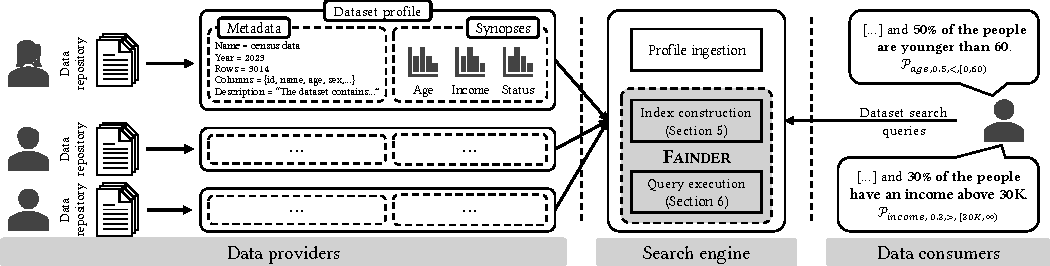
\includegraphics[scale=1]{figures/diagrams/problem_overview.pdf}
    \caption{
        Schematic overview of distribution-aware dataset search and \system{}'s role in it: Data providers offer public dataset profiles used by search engines to answer dataset search queries with distributional requirements effectively and efficiently.
    }
    \Description{Schematic overview of distribution-aware dataset search.}
    \label{fig:problem_overview}
    % Max figure width: 17.79cm
    % Max figure height: 4.5cm
    % NOTE: We place this figure here because it appears too late in the text otherwise
    \vspace{-1em}
\end{figure*}

We start by introducing basic definitions about decentralized data repositories and presenting the notation we use throughout the paper (summarized in Table~\ref{tab:notation_overview}).

\paragraph{Dataset}
A dataset is a collection of related observations organized and formatted in a particular way~\cite{chapman_dataset_2020}.
In this paper, we focus on tabular datasets that contain at least one numerical column, as they are both widespread and of particular interest when searching for datasets that meet distributional requirements.

\begin{definition}[\textsc{Tabular Dataset}]
    A tabular dataset $D$ with a schema $\cA \equiv \langle A_1,\ldots, A_l \rangle$ consists of  $l$ columns and a collection of tuples $T$ such that $t\in T$ contains $l$ values.
\end{definition}

We refer to the $i^{\text{th}}$ column of a dataset $D$ as $D[i]$.
Each dataset (and its columns) is often accompanied by specific metadata used for dataset search.
For example, Google Dataset Search~\cite{noy_google_2019} allows searching through textual dataset descriptions, while Auctus~\cite{castelo_auctus_2021} also supports search over column names and their types.
Other examples of metadata include row counts or spatiotemporal information.
We refer to these joint characteristics as dataset profiles.

\begin{definition}[\textsc{Dataset Profile}]
    A dataset profile $P_D$ is defined as the properties or constraints the tuples in $D$ satisfy.
\end{definition}

A dataset profile may contain any dataset description, such as column headers, row counts, or licenses~\cite{abedjan_profiling_2015}.
We assume that $P_D$ includes column identifiers, histograms of numerical columns, and the unit of measurement of the histogram elements.
Histograms are widely used in data management:
Database systems, such as PostgreSQL, use them for query optimization~\cite{cormode_synopses_2011}, while dataset search engines, such as Auctus~\cite{castelo_auctus_2021}, use them to visualize dataset contents.
Since data owners can decide for which columns they want to enable distribution-aware search and share histograms, we consider them a low-barrier synopsis for enriching dataset profiles.

\paragraph{Histogram}
A histogram is an approximate data synopsis that discretizes a value collection into different bins and stores the frequency of the values that fall into each bin~\cite{cormode_synopses_2011}.
Without loss of generality, we assume that histograms contain relative frequencies (i.e.,~densities) and that histogram bins are non-overlapping.

There are numerous ways to compute a histogram on top of the values in a dataset~\cite{cormode_synopses_2011}.
Our setting is agnostic to the details of histogram creation, as dataset search engines must handle a heterogeneous set of dataset profiles provided by data owners.
Consequently, we define a histogram $H_{D[i]}$ over a column $D[i]$ as a list of tuples $\langle b, v\rangle$, where bin $b \equiv [b_l, b_h)$ denotes an interval over the values in $D[i]$ and $v$ denotes the density of values in $b$.
We use \edges{$H_{D[i]}$} to refer to the list of all bin edges for the histogram $H_{D[i]}$ and \density{$H_{D[i]}$} for the corresponding list of densities.
The subscript $D[i]$ is ignored whenever it is clear from the context.

\paragraph{Data Repository}
We consider a setting where different entities (often called data providers) have their own set of datasets.
A collection of datasets $\cD=\sset{D_1,\ldots, D_k}$, gathered by one or multiple data providers, is called a data repository.
Each data repository independently computes synopses (histograms for our setting) along with other metadata of its datasets and shares them with a search engine.
To support dataset search, the search engine processes these synopses, collates a collection of histograms $\cH =\sset{H_1,\ldots, H_n}$, and evaluates user queries with it to identify relevant datasets.

%!TEX root = ../main.tex

\section{Distribution-Aware Dataset Search}
\label{sec:problem}

We formalize the problem of distribution-aware dataset search over decentralized data repositories and discuss its research challenges.

\subsection{Problem Definition}
\label{sec:problem_definition}

Figure~\ref{fig:problem_overview} provides a semantic overview of the distribution-aware dataset search setting.
Based on the data market terminology by \textcite{asudeh_towards_2022}, we consider the passive-provider model, where data owners provide information about their datasets to search engines, and users come to a search engine to find relevant datasets.
We assume that users have complex search needs consisting of multiple requirements about the data they seek.
Specifically, we focus on distributional requirements.
In the following, we introduce our query model and formalize the search problem.

\paragraph{Predicate}
We model a user's search query as a Boolean predicate that can be checked with respect to any dataset or its corresponding profile.
Specifically, we consider \emph{keyword-based predicates}, denoted by $\cK_w(D)$, that hold when $D$'s profile contains the specified keyword $w$.
For example, the predicate ``\textit{title} = `census' '' returns true for all datasets whose title field contains ``census''.
In contrast, the simpler predicate ``cancer'' returns true whenever the word ``cancer'' appears anywhere in the dataset profile.
To enable distribution-aware dataset search, we additionally consider percentile predicates.

A \emph{percentile predicate} specifies the condition for a specific distributional requirement.
We define the predicate using the notions of \emph{column identifier} $C$, \emph{fraction} $ 0 < p \leq 1$, \emph{comparison operator} $\theta \in \sset {<, \leq, >, \geq}$, and \emph{range} $r \equiv [r_l, r_h)$, where $r_l, r_h \in \bR$ and $r_l < r_h$.
For a given $C$, $p$, $\theta$, and $r$, the predicate $\cP_{C, p, \theta, r}(D)$ defined on a dataset $D$ holds whenever the dataset contains a column matched by $C$ and the comparison $p \: \theta \: f$ is true, where $f$ is the fraction of values in the column that lie within the range $[r_l, r_h)$.
Other range definitions are possible but omitted for the sake of brevity.
More formally:
\[
\cP_{C, p, \theta, r}(D) \coloneq
\begin{cases}
    \true   & \text{if } \exists D[i]: \\
            & (D[i] \in C) \land \left(p \; \theta \; \frac{|\{x: x\in D[i] \land x\in [r_l,r_h)\}|}{|D[i]|}\right) \\
    \false  & \text{otherwise}
\end{cases}
\]
The column identifier $C$ can be a simple string or a more complex operation, such as a column match based on semantic similarity~\cite{zhang_ad_2018}.
In simple words, the predicate $\cP_{\text{age},0.5,\leq,[0,60)}(D)$ holds if \textit{``dataset $D$ has a column `age' and at least 50\% of the people are younger than 60''}.
However, a key challenge of evaluating percentile predicates over decentralized data repositories is that the search engine only has access to dataset profiles instead of raw data.
Therefore, we must design solutions capable of evaluating $\cP(P_D)$ rather than $\cP(D)$.\looseness=-1


\begin{table}[t]
    % NOTE: We place the table here to show it at a more convenient location in the text.
    \centering
    \footnotesize
    \caption{Notation overview.}
    \label{tab:notation_overview}
    \addtolength{\tabcolsep}{-0.5em}
    \begin{tabular}{cl cl cl}
        \toprule
        Symbol & Meaning                & Symbol  & Meaning            & Symbol & Meaning \\
        \midrule
        $D$    & Dataset                & $b$     & Histogram bin      & $n$    & \#~histograms \\
        $\cD$  & Dataset collection     & $c$     & Cluster            & $\cI$  & \system{} index \\
        $P_D$  & Dataset profile of $D$ & $k$     & \#~clusters        & $Q$    & Query \\
        $H$    & Histogram              & $\cB$   & Bin budget         & $\cK$  & Keyword pred. \\
        $H'$   & Aligned histogram      & $\cB_c$ & Bin budget for $c$ & $\cP$  & Percentile pred. \\
        $\cH$  & Histogram collection   & $\cH_c$ & Histograms in $c$  & $S$    & Result set \\
        \bottomrule
    \end{tabular}
\end{table}

\paragraph{Query}
A query $Q$ is a Boolean combination of keyword and percentile predicates.
Keyword-based dataset search has been extensively studied in the literature~\cite{chapman_dataset_2020, noy_google_2019, wei_survey_2013, zhang_ad_2018}.
Here, we focus on supporting distribution-aware search with $Q(D) \equiv \cP(D)$.

We now define the distribution-aware dataset search problem.

\begin{problem}[\textsc{Distribution-Aware Dataset Search}]
    Given a collection of data sources $\cS$, such that each source $s$ has a data repository $\cD_s = \sset{D_1,\dots, D_d}$ and shares corresponding dataset profiles $\cM_s = \sset{P_{D_1},\dots, P_{D_d}}$, and a dataset search query $Q$, find the set of datasets $S = \sset{D: D\in \cD \text{ and } Q(P_D)\text{ holds}}$.
\end{problem}

\subsection{Research Challenges}
\label{sec:research_challenges}

Of the three challenges presented in Section~\ref{sec:intro}, we address C1 by using histograms and C2 by proposing percentile predicates.
We now discuss the difficulties of designing a fast and accurate solution for evaluating percentile predicates on histograms~(C3).
Across all stakeholders, the desiderata for a distribution-aware dataset search engine are: (1)~interactive query execution time with sublinear scaling in the number of datasets, (2)~accurate results, and (3)~a minimal resource (i.e.,~memory) footprint of any data structures other than dataset profiles.
These three dimensions form a triangle with a performance trade-off since we cannot maximize all dimensions simultaneously: producing accurate results in minimal time requires precomputation, which implies higher memory usage; accurate results without additional memory usage require an iterative execution with linear runtime; and returning results in sublinear time with minimal memory usage effectively means guessing with arbitrary accuracy.
Therefore, at least one dimension will always perform worse than if we solely optimized a solution for it.
Beyond this trade-off, a central challenge of our problem is the handling of heterogeneous histograms provided by the data owners.

\paragraph{Predicate Evaluation With Histograms}
In principle, evaluating a percentile predicate using a histogram $H$ is straightforward, as its bin edges and densities include the required information.
Consider the exemplary histograms from Figure~\ref{fig:example_histograms_1} and our predicate $\cP_{\text{age}, 0.5, \leq, [0, 60)}$, looking for datasets where at least 50\% of the people are younger than 60.
To evaluate it, we sum up the density $f$ of all bins that fall into $[r_l, r_h)$.
For $H_a$, we have $f=0.6$; thus, the predicate holds.
Likewise, it is straightforward to see that $\cP$ does not hold for $H_b$.
Yet, the triviality of this example does not extend to decentralized data repositories, as each data provider independently creates histograms of their data at will so that a bin may only partially overlap with $[r_l, r_h)$, such as in the case of histogram $H_c$.\looseness=-1

Evaluating a predicate on heterogeneous histograms often requires estimating a bin's contribution to $f$.
There are several intra-bin value distribution estimation strategies~\cite{cormode_synopses_2011}.
Common strategies are to underestimate (ignore bin $b$), overestimate (add the total density of $b$), or assume a continuous value distribution and add a share of $b$'s density proportional to the overlap with range $r$.
Unless we overestimate $f$ for $\theta =$``<'' and underestimate it for $\theta =$``>'', we risk filtering out dataset columns that match the predicate.
Since a histogram is a lossy representation of $D$, this approach may produce false positives (a limitation of synopsis-based dataset search).
However, the approach guarantees full recall, a crucial requirement to ensure effectiveness.
If full recall is not required, the estimation could be changed to achieve full precision or to maximize $F_1$ score.

\begin{figure}[t]
    \centering
    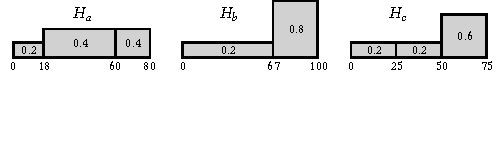
\includegraphics[trim=0 1.35cm 0 0]{figures/diagrams/example_histograms.pdf}
    \caption{Histograms $\boldsymbol{H_a}$, $\boldsymbol{H_b}$, and $\boldsymbol{H_c}$.}
    \Description{Three exemplary histograms to underscore research challenges.}
    \label{fig:example_histograms_1}
    % Max width: 241.14749pt / 8.47cm
\end{figure}

\paragraph{Predicate Evaluation Over Dataset Collections}
A simple yet effective way to evaluate a percentile predicate at the dataset collection level is a technique we call \pscan.
It iterates through each histogram $H$, determines the bins that fall into the range $r$, and adds $H$ to the result set $S$ if the predicate is fulfilled.
This makes it an accurate and memory-efficient solution, as it uses no additional data structures.
However, a major limitation is that it scales linearly in the number of histograms.
Even though \pscan can filter the histogram collection based on column identifier $C$, a significant number of histograms can remain after filtering.
For example, Kaggle~\cite{kaggle_inc_kaggle_2024} has more than $15\:000$ datasets that match the keyword ``age'' and more than $23\:000$ datasets matching the query ``date'' as of February 2024.
This problem becomes exacerbated if users pose generic column identifier predicates instead of keywords, such as \textit{``match any column related to finance''}.
Thus, \pscan leaves a need for a fast and accurate as well as a fast and resource-efficient solution, which we address in this paper.

% Practical problems
The critical problem for the sublinear scalability of percentile predicate evaluation is the heterogeneity of histograms from decentralized data repositories.
As the histograms have different numbers and distributions of bins, we must individually identify the bins within a predicate's range per histogram.
Allowing arbitrary value ranges in a predicate further complicates the problem since an infinitely large number of possible ranges must be considered for an index.
If we instead require that either $r_l = -\infty$ or $r_h = \infty$, we can achieve orders of magnitude speedups for percentile predicates with intelligent precomputation.
Such ``one-sided'' intervals for specifying a range enable us to execute queries similar to the ones in our motivating example.
Assuming that $r_l = -\infty$ or $r_h = \infty$, the range $r$ of a predicate effectively cuts the number line into two parts.
Consequently, we can rewrite any predicate with $r_l = -\infty$ into a predicate with $r_h = \infty$ (and vice versa) by setting $r_l = r_h$, replacing $p$ with $1-p$ and flipping the comparison operator $\theta$.
Without loss of generality, we therefore assume $r_l = -\infty$ and simplify the notation of a percentile predicate to $\cP_{C, p, \theta, r_h}(P_D)$ for the rest of this paper.

%!TEX root = ../main.tex

\section{Fainder}
\label{sec:index_overview}

We propose \system{}, an index for percentile predicates that attains robust scalability and accurate (optionally exact) results to address the identified research challenges.
This section gives an overview of \system{}'s architecture.
Subsequently, we discuss the technical details of index construction and querying in Sections~\ref{sec:index_construction} and~\ref{sec:index_querying}.

\paragraph{Key Insights}
The central intuition behind \system{} is that whenever all histograms have the same set of bins, we can precompute a subset of cumulative densities to answer percentile predicates efficiently with sublinear time complexity.
Conceptually, we achieve a logarithmic scaling by sorting the histograms' cumulative densities at each bin boundary and using a two-stage binary search over the bins and densities to identify the result set.
In practice, however, histogram heterogeneity prevents us from directly using binary search on a collection.
To overcome this limitation, \system{} homogenizes histograms by mapping them to a collection-wide consistent bin distribution.
Changing the bin edges of a histogram and reassigning a bin's density to one or multiple new bins is inherently approximate.
Thus, we must ensure that \system{} has high accuracy comparable to \pscan during index construction.
Naive approaches to creating such a global distribution are constructing the union of all original bin edges or creating $\epsilon$-sized bins between the minimum and maximum value of a collection.
However, these approaches lead to an excessive memory footprint or subpar result accuracy, as we show with a concrete example in Section~\ref{sec:clustering}.
\system{} addresses these challenges by creating a clustered global bin distribution instead.
Empirical evaluation on one million datasets (GitTables~\cite{hulsebos_gittables_2023}) shows that our clustering approach reduces the memory footprint from more than one TB to 3.2 GB without a substantial increase in runtime while maintaining high accuracy.

\paragraph{System Overview}

\begin{figure}[t]
    \centering
    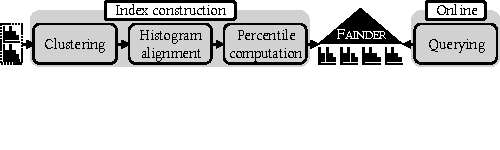
\includegraphics[trim=0 1.4cm 0 0]{figures/diagrams/fainder.pdf}
    \caption{Overview of \system{}.}
    \Description{Schematic system overview that describes the different stages of \system{}.}
    \label{fig:fainder_overview}
    % Max width: 241.14749pt / 8.47cm
\end{figure}

Figure~\ref{fig:fainder_overview} summarizes the lifecycle of \system{}.
The starting point is a histogram collection $\cH$ and a mapping $\FuncSty{column}(H)$ that projects each histogram to its associated column identifier.
At first, \system{} clusters $\cH$ based on the bin edges of each histogram.
As part of the clustering phase, we must decide what share of the global bin budget (i.e.,~memory budget) we assign to each cluster and how the bin edges within a cluster should be distributed.
Next, \system{} aligns the histograms $\cH_c$ in a cluster $c$ by distributing the original bin density $\density{H}$ to $\density{H'}$ based on the cluster bins $\edges{\cH_c}$.
For this, we introduce two alternative histogram alignment techniques, rebinning and conversion, that offer different trade-offs for precision, recall, and index size.
Having aligned all histograms in a cluster, \system{} indexes them by precomputing and sorting the cumulative density per histogram and bin.
Finally, \system{} evaluates percentile predicates using binary search at query time.
Like any search index, \system{} amortizes its additional memory consumption and one-time construction cost through repeated execution time savings each time it evaluates a predicate.
We discuss the conceptual index maintenance costs in Section~\ref{sec:percentile_computation} and experimentally evaluate them in Section~\ref{sec:micro_benchmarks}.\looseness=-1

\paragraph{Index Variants}

\begin{figure}[t]
    \centering
    \begin{forest}
    forked edges,
    for tree={
        font=\scriptsize,
        draw,
        rounded corners=2pt,
        align=center,
        inner sep=2pt,
        edge={font=\scriptsize, -stealth},
        calign=center,
        l sep=0.1em,
        s sep-=1pt,
        fork sep=0.5em,
    }
    [{Do you require exact query results?}
        [{Do you have a tight memory budget?}, edge label={node[midway,left] {No}}
            [{Use \approximate{} with\\rebinning-based alignment.}, edge label={node[midway,left] {Yes}}, tier=rec]
            [{Use \approximate{} with\\conversion-based alignment.}, edge label={node[midway,right] {No}}, tier=rec]
        ]
        [{Use \exact{} with\\conversion-based alignment.}, edge label={node[midway,right] {Yes}}, tier=rec]
    ]
    \end{forest}
    \caption{Flowchart for choosing a \system{} variant.}
    \Description{Questions for choosing a \system{} variant.}
    \label{fig:index_variants}
\end{figure}

The two histogram alignment techniques enable us to design three unique \system{} variants that cater to different requirements.
Figure~\ref{fig:index_variants} summarizes them with guidelines for choosing an appropriate version.
If exact results are not required or execution time is paramount, rebinning and conversion offer two alternative \approximate{} variants.
While rebinning minimizes the index size and construction time, conversion allows users to select a full precision or recall guarantee at query time.
Thus, \exact{} utilizes a conversion-based index to efficiently prune the search space before conducting \pscan on a small subset of histograms.
Note that a conversion-based index can be used for both approximate and exact results based on the runtime preference per query.
Therefore, the primary decision during index construction is to choose either rebinning- or conversion-based histogram alignment.\looseness=-1


\section{Index Construction}
\label{sec:index_construction}

We discuss the construction of \system{}, which consists of the steps clustering, histogram alignment, and percentile computation.\looseness=-1

\subsection{Clustering}
\label{sec:clustering}

The clustering phase computes a feature vector for each histogram, clusters them, and defines the aligned bins for each cluster.
The motivation for this phase are the bin width and value range differences between histograms in a dataset collection.
To illustrate this, consider the histogram collection from Figure~\ref{fig:example_histograms_2}, which we use as a running example throughout this section, and assume that there is another histogram $H_5$ with $\edges{H_5} = [-100, -85, -70]$ (not depicted for brevity).
The global value range of this collection is [-100, 100].
However, no histogram covers the interval (-70, 0).
Therefore, allocating bins in the global bin distribution for this region would be a waste of space, as there are no density changes.
Furthermore, $H_1$ and $H_4$ both cover the interval [0, 3] but with vastly different bin widths.
Thus, converting $\edges{H_1}$ and $\edges{H_4}$ to a joint bin distribution would be too detailed for $H_1$ or too coarse for $H_4$.
Considering that \system{} should have a minimal memory footprint, aligned bins must only cover relevant parts of the global value range with a locally appropriate bin width to achieve accurate query responses efficiently.
Since we do not know user queries in advance, an optimal solution is query-agnostic and minimizes the information loss between original and global bins, given a user-defined bin budget $\cB$.
Formally, we consider the overlap of each original bin $b_i \equiv [b_{il}, b_{ih})$ with the closest global bin $b_j^g$ as a proxy for mitigating information loss and thus aim to maximize it:
\begin{equation}
\label{eq:overlap_optimization}
\underset{b^g}{\FuncSty{argmax }} O = \mathcolor{brown!80}{\sum_{i}} \mathcolor{red!70}{\underset{j}{\FuncSty{max}}} \left( \frac{\mathcolor{red!70}{\FuncSty{max} \left(\FuncSty{min}(b^{}_{ih}, b^g_{jh}) - \FuncSty{max}(b^{}_{il}, b^g_{jl}), 0\right)}}{\mathcolor{blue!70}{\FuncSty{max}\left(\FuncSty{width}(b_i), \FuncSty{width}(b_j^g)\right)}} \right)
\end{equation}
The cumulative overlap $O$ reflects the overlap between an original bin and the most closely fitting global bin (red), normalized by the bin width (blue), and summed across original bins (brown).
If we consider each possible global bin as a unit-weight item whose value is its marginal improvement of $O$, finding an optimal solution with a limited number of bins is a variation of the knapsack problem (i.e.,~NP-hard).
Therefore, we use a three-step procedure based on clustering to break down the global bin definition problem into smaller parts and efficiently find an approximate solution.

\begin{figure}[t]
    \centering
    \begin{tikzpicture}
        \node(H1) {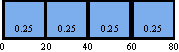
\includegraphics[page=1, scale=1]{figures/diagrams/histograms.pdf}};
        \node(H2) [right=15mm of H1.south east, anchor=south west] {\includegraphics[page=3, scale=1]{figures/diagrams/histograms.pdf}};
        \node(H3) [below=0mm of H1.south west, anchor=north west] {\includegraphics[page=4, scale=1]{figures/diagrams/histograms.pdf}};
        \node(H4) [right=15mm of H3.south east, anchor=south west] {\includegraphics[page=2, scale=1]{figures/diagrams/histograms.pdf}};

        \node[left=0mm of H1, inner sep=0mm] {$H_1$};
        \node[left=0mm of H2, inner sep=0mm] {$H_2$};
        \node[left=0mm of H3, inner sep=0mm] {$H_3$};
        \node[left=3mm of H4, inner sep=0mm] {$H_4$};

        \node [bound, fit margins = {left=9pt,right=3pt, bottom=0pt,top=5pt}, fit=(H1) (H3)] {$\cH_1$};
        \node [bound, fit margins = {left=9pt,right=2pt, bottom=0pt,top=0pt}, fit=(H2) (H4)] {$\cH_2$};
    \end{tikzpicture}
    \caption{Histograms $H_1$--$H_4$ and clusters $\cH_1, \cH_2$.}
    \Description{A set of four example histograms used throughout Section~\ref{sec:index_construction}.}
    \label{fig:example_histograms_2}
    \vspace{0.6em}
\end{figure}

\paragraph{Clustering Features}
Clustering aims to partition the histogram collection $\cH$ into sets of histograms that cover similar value ranges with similar bin widths.
Therefore, we compute a feature vector
\[
\boldsymbol{v}_{H} = \begin{bmatrix}\FuncSty{min}(\edges{H}) & \FuncSty{max}(\edges{H}) & \FuncSty{avgWidth}(\edges{H})\end{bmatrix}
\]
for each histogram, where \FuncSty{avgWidth} represents the average bin width of a histogram.
Due to the heterogeneity of histograms, directly clustering the feature vectors would yield suboptimal results.
Therefore, we preprocess them with a non-linear quantile transform~\cite{pedregosa_scikit-learn_2011}, which maps all features to a uniform distribution on the interval $[0, 1]$ to reduce the impact of outliers.
The intuition for this transformation is to make the different value scales of our features more directly comparable while being robust to outliers.

\paragraph{Clustering Algorithm}
\system{} requires a scalable clustering algorithm to partition all histograms into reasonable, ideally balanced clusters.
Conceptually, the clustering algorithm choice is a hyperparameter of \system{} and orthogonal to the other stages.
Concretely, we use k-Means~\cite{lloyd_least_1982} for clustering and discuss our investigation of alternative clustering algorithms in Section~\ref{sec:solution_effectiveness}.

\paragraph{Cluster Bin Assignment}

\begin{figure}[t]
    \begin{tikzpicture}
        \node(H13) {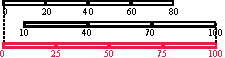
\includegraphics[page=1]{figures/diagrams/fainder_overview.pdf}};
        \node(H1) [above left=-4mm and -2mm of H13] {\small $H_1$};
        \node(H2) [below=-0.8mm of H1] {\small $H_3$};
        \node(CH1) [below=-0.8mm of H2] {\small $\cH_1$};

        \node(H24) [right = 5mm of H13] {\includegraphics[page=4]{figures/diagrams/fainder_overview.pdf}};
        \node(H4) [above left=-4mm and -2mm of H24] {\small $H_4$};
        \node(H2) [below=-0.8mm of H4] {\small $H_2$};
        \node(CH2) [below=-0.8mm of H2] {\small $\cH_2$};
    \end{tikzpicture}
    \caption{Cluster bin assignment for $\cH_1$ and $\cH_2$ ($\cB=8$).}
    \Description{A visual summary of histogram clustering based on the histogram bin edges and subsequent cluster bin assignment.}
    \label{fig:bin_assignment}
\end{figure}

\begin{figure}[t]
    \subfloat[$H_1 \to H'_1$]{
        \includegraphics[page=2]{figures/diagrams/fainder_overview.pdf}
    }%
    \hfill%
    \subfloat[$H_2 \to H'_2$]{
        \includegraphics[page=6]{figures/diagrams/fainder_overview.pdf}
    }

    \subfloat[$H_3 \to H'_3$]{
        \includegraphics[page=3]{figures/diagrams/fainder_overview.pdf}
    }%
    \hfill%
    \subfloat[$H_4 \to H'_4$]{
        \includegraphics[page=5]{figures/diagrams/fainder_overview.pdf}
    }
    \caption{Rebinning-based histogram alignment. The aligned histogram bins and densities are shown in red.}
    \Description{An example of the rebinning procedure based on the histograms from Figure~\ref{fig:example_histograms_2} and cluster bins from Figure~\ref{fig:bin_assignment}.}
    \label{fig:rebinning_alignment}
\end{figure}

After clustering, we must distribute the global bin budget $\cB$ across clusters.
Figure~\ref{fig:bin_assignment} demonstrates this final step of the clustering phase with our running example.
The simplest method is to assign a budget proportional to the cluster size:\looseness=-1
\begin{equation}
\label{eq:cluster_bin_budget}
\cB_c =  \FuncSty{max}\left(1, \left\lfloor \cB \frac{|\cH_c|}{\sum_{i=1}^k |\cH_i|} \right\rfloor \right)
\end{equation}
However, in the worst case, this results in small clusters only consisting of a single bin, whereas large clusters might receive a much more fine-grained bin width than needed.
Therefore, we use additive smoothing~\cite{manning_introduction_2008} to anneal the proportional bin budget towards a uniform assignment based on the parameter $\alpha$.
Given a cluster (value range) and bin budget, we create equi-width bins $\edges{\cH_c}$ for each cluster.
Conceptually, the cluster bin assignment strategy is a hyperparameter that a search engine operator can adapt.
For example, we could instead allocate the same bin budget to each cluster or choose an individual bin definition algorithm for each cluster, such as equi-height bins (which are more costly to compute).


\subsection{Histogram Alignment}
\label{sec:alignment}

Given a cluster of histograms $\cH_c$ and its cluster bins $\edges{\cH_c}$, the task of histogram alignment is to transform each $H \in \cH_c$ to $H'$, such that $\density{H'}$ represents the original value distribution of $H$ on $\edges{\cH_c}$.
This requires distributing the density of each original bin to one or multiple new bins.
Consequently, histogram alignment requires approximating the data distribution within a bin and strongly influences the downstream index accuracy.

We present two alternative approaches for histogram alignment that offer different trade-offs between index accuracy and resource requirements.
Rebinning aims to minimize the index size but does not provide a formal accuracy guarantee.
It allows the system operator to make an assumption about the intra-bin value distribution and will balance precision and recall if the assumption holds.
While rebinning is an intuitive and efficient way to align histograms, there are scenarios where guaranteeing total precision or recall is critical.
For example, precision is essential if users only want to review a few guaranteed true results.
Contrarily, total recall is crucial to use \system{} as a pruning tool for an exact solution.
Thus, conversion ensures total recall or precision at query time but requires additional storage compared to rebinning.

\paragraph{Rebinning}
The principal idea of rebinning is to compute the overlap interval $o_{ij} = [\FuncSty{max}(b_{il}, b_{jl}), \FuncSty{min}(b_{ih}, b_{jh}))$ between all pairs of bins $b_i$ from the original histogram and $b_j$ from the respective cluster bins.
Given $o_{ij}$, we compute the fraction of the original bin's density $\density{H}[i]$ that lies within $o_{ij}$ and add it to $\density{H'}[j]$.
Since a histogram does not contain information about the distribution of values within a bin, rebinning must approximate this fraction if $o_{ij} \neq b_i$.
The simplest intra-bin density estimation assumes a uniform value distribution within a bin (i.e.,~we add $\tfrac{\FuncSty{width}(o_{ij})}{\FuncSty{width}(b_i)}\%$ of $b_i$'s density to $b_j$)~\cite{cormode_synopses_2011}.
However, a search engine can make other assumptions about the data distribution.
For instance, cubic spline interpolation is a more costly alternative but can better estimate non-uniform value distributions.

Figure~\ref{fig:rebinning_alignment} continues our running example and shows how to rebin $H_1$--$H_4$ based on the cluster bins.
For example, the fourth bin of $H_2$ has the range $[5,\;8]$.
Thus, its overlap with $\cH_2[2]$ is $o_{32} = [5,\;6)$.
Under a continuous value assumption, this means that one-third of $H_2[3]$'s density (0.1) is assigned to $\density{H'_2}[2]$, which, together with the contributions from $H_2[2]$, has a total density of 0.3.

\paragraph{Conversion}

The central intuition of conversion-based histogram alignment is to compute a lower and upper bound for the density at each bin.
To compute these bounds, we create a \textit{conversion matrix} $CM$ for every array pair ($\edges{H}$, $\edges{\cH_c}$) of original bins and cluster bins.
$CM$ is a Boolean matrix that is true for each bin pair that partially or fully overlaps.
Based on $CM$, we know which original bin \textit{might} or \textit{must} contribute to the density of any bin in $H'$.
Since the original and cluster bins form an n:m relationship, we cannot assume that the upper bound of $H'[i]$ is the lower bound of $H'[i+1]$.
This requires us to store two numbers per bin, resulting in a $2\times$ index size compared to rebinning.
At the same time, conversion enables predicate evaluation with full precision or recall, as we do not perform any intra-bin estimation but fully add $\density{H}[i]$ to $\density{H'}[j]$ if it contributes to the lower or upper bound of the bin's density.
Depending on the comparison operator in a predicate, \system{} uses the respective density bound to prevent false positives or negatives.
Given a query, such as ``at least 50\% of the values are lower than 60'' with a total recall requirement, the upper density bound lets us filter out those histograms that do not have a cumulative density higher than 50\% in the bin where 60 lies.

Figure~\ref{fig:conversion_alignment} shows the conversion matrix for histogram $H_2$ and cluster $\cH_2$ on the left.
On the right, we visualize the bin-wise conversion of $H_2$.
In practice, we do not convert each bin separately but directly compute the lower and upper bounds for the cumulative density of a bin.
By knowing which cluster bins an original bin partially contributes to, we also know that this bin must fully contribute to the cumulative density of all following cluster bins, highlighted by the green lower bound area.
The orange upper bound area consists of the lower bound area and the bins whose contribution is unclear.
We compute the cumulative bounds by summing up the density of all original bins that contribute to a cluster bin's lower or upper bound.
The cumulative density of $H'_2[2]$, for example, is bounded by $[0.5,\:1]$ since the first two bins of $H_2$ (green area) fully contribute to the bin's density.
In contrast, the orange area (bins 1-4) comprises the original bins that might contribute to the cumulative density of $H'_2[2]$.\looseness=-1

\begin{figure}[t]
    \begin{tikzpicture}[anchor=north west, every node/.style={font=\scriptsize}]
        \matrix(mat) [
        nodes=draw,minimum width=6mm,
        column sep=0mm,
        font=\small,
        ]
        {
        \node(11) {1};   & \node(12){1};     & \node(13){0};      & \node(14){0}; \\
        \node(21) {0};   & \node(22){1};     & \node(23){0};      & \node(24){0}; \\
        \node(31) {0};   & \node(33){0};     & \node(33){1};      & \node(34){0}; \\
        \node(41) {0};   & \node(42){0};     & \node(43){1};      & \node(44){1}; \\
        };

        \begin{pgfonlayer}{background}
        \foreach \x in {11,12,13,14,22,23,24,33,34,43,44}
        \filldraw[DarkOrange!60][] ($(\x.north west)+(0.1ex, -0.1ex)$) -- ($(\x.south west)+(0.1ex, 0.1ex)$) -- ($(\x.south east)+(-0.1ex, 0.1ex)$)--cycle;

        \foreach \x in {13,14,23,24,34}
        \filldraw[ForestGreen!60][] ($(\x.north west)+(0.2ex, -0.1ex)$) -- ($(\x.north east)+(-0.1ex, -0.1ex)$) -- ($(\x.south east)+(-0.1ex, 0.15ex)$)--cycle;
        \end{pgfonlayer}

        \node[left=8mm of mat, rotate=90, anchor=north] {$\edges{H_2}$};
        \node[above=1.5mm of mat] {$\edges{\cH_2}$};

        \node[above=0mm of 11] {[0,2)};
        \node[above=0mm of 12] {[2,4)};
        \node[above=0mm of 13] {[4,6)};
        \node[above=0mm of 14] {[6,8]};

        \node[left=0mm of 11] {[1,3)};
        \node[left=0mm of 21] {[3,4)};
        \node[left=0mm of 31] {[4,5)};
        \node[left=0mm of 41] {[5,8]};

        \node(H2)[right=1mm of mat.south east, anchor=south west] {\includegraphics[page=9]{figures/diagrams/fainder_overview.pdf}};

        \node[below=-1mm of mat] {$CM(H_2, \cH_2)$};
        \node[below=-1mm of H2] {$H_2 \to H'_2$};

        \node[draw, fill=DarkOrange!60, minimum width=1mm, left=12mm of mat.south west, anchor=south] (ub) {};
        \node[draw, fill=ForestGreen!60, minimum width=1mm, left=2mm of ub.south west, anchor=south] (lb) {};
        \node[above=0.5mm of lb.north, anchor=west, rotate=90] {\scriptsize\itshape Lower bound};
        \node[above=0.5mm of ub.north, anchor=west, rotate=90] (ubtext) {\scriptsize\itshape Upper bound};
        \node[draw, dashed, fit margins = {left=1pt,right=0pt,bottom=1pt,top=1pt}, fit=(lb)(ubtext)] {};
    \end{tikzpicture}
    \captionsetup{belowskip=0.0em, aboveskip=-0.3em}
    \caption{Conversion-based histogram alignment: (left) conversion matrix for computing percentile bounds, (right) aligned histogram with lower and upper bounds in red.}
    \Description{An example of the conversion procedure based on histogram $H_2$ from the example histograms.}
    \label{fig:conversion_alignment}
    \vspace{-0.3em}
\end{figure}

\subsection{Percentile Computation}
\label{sec:percentile_computation}

\begin{figure}[t]
    \centering
    \begin{tikzpicture}
        \node(H1) {\includegraphics[page=7,scale=0.86]{figures/diagrams/fainder_overview.pdf}};
        \node(H2) [right=1.5mm of H1.north east, anchor=north west] {\includegraphics[page=8,scale=0.86]{figures/diagrams/fainder_overview.pdf}};
        \node [bound, fit margins = {left=-1pt,right=-1pt, bottom=0pt,top=-1pt}, fit=(H1), label={[anchor=south west, inner sep=2pt, text=gray]south west:$\cH_1$}] {};
        \node [bound, fit margins = {left=-1pt,right=-1pt, bottom=0pt,top=-1pt}, fit=(H2), label={[anchor=south east, inner sep=2pt, text=gray]south east:$\cH_2$}] {};

        \path (H1.north) -- (H2.north) node[inner sep=1pt, yshift=2pt, midway] (ab) {\scriptsize\itshape Aligned bin edges};
        \path (H1.east) -- (H2.west) node[inner sep=1pt, yshift=-12pt, midway] (cd) {\scriptsize\itshape Cumulative densities};

        \draw[-, thick] (H1.north) |- (ab) -| (H2.north);
        \draw[-, thick] ([yshift=-7pt]H1.center) |- (cd) -| ([yshift=-7pt]H2.center);
        \draw[-, thick] ([yshift=8pt, xshift=30pt]H1.south) -- node[inner sep=1pt, fill=white]{\scriptsize\itshape Histogram pointers} ([yshift=8pt, xshift=-30pt]H2.south);
    \end{tikzpicture}
    \caption{Rebinning-based \system{} index for $H_1$--$H_4$. Red color outlines evaluating the predicate \textit{``at least 65\% of the values are less than 50''}. Dashed arrows are histogram pointers.\looseness=-1}
    \Description{A visualization of index construction and querying.}
    \label{fig:percentile_computation_and_querying}
    \vspace{-0.4em}
\end{figure}

The percentile computation phase consists of initialization, density summation, and sorting.
We demonstrate its result in the upper part of Figure~\ref{fig:percentile_computation_and_querying}.
For each cluster $c$, \system{} creates a $(n_c \times \cB_c)$ array to store percentiles and a pointer array of the same size to keep a reference to the respective histograms.
For conversion-based indices, this array pair is created twice for the lower and upper percentile bounds.
Next, \system{} computes the cumulative density per cluster bin and histogram.
Since all histograms in a cluster have the same bins, \system{} uses vectorization to compute the cumulative sums efficiently and stores them in the percentile array.
Lastly, we sort the percentile array and corresponding pointers column-wise.
This way, \system{} knows that all histogram pointers after a given one in the current bin have an equal or higher cumulative density.\looseness=-1

\paragraph{Index Size and Maintenance Costs}
\system{}'s query execution time improvements must justify its overhead, specifically the memory consumption and maintenance cost.
Without clustering, \system{}'s asymptotic space complexity is $O(n \cB)$, as we must store a percentile-pointer pair for each histogram and global bin.
However, with clustering, we do not have to process the full Cartesian product of histograms and bins across clusters, making construction faster and the index smaller.
The more clusters an index has, and the more evenly balanced they are, the smaller the size of \system{}.
In the case of a perfectly even distribution, the size shrinks to $O(\frac{n \cB}{k})$.

The maintenance costs of \system{} are divided into one-time construction costs and repeated histogram insertion and deletion costs.
Since we have to initially cluster and individually align each histogram, the construction costs scale linearly with $n$.
However, these costs are mitigated by the fact that an index is seldom created but often queried.
More importantly, we can insert into and delete from \system{} at minimal cost since histogram alignment is an incremental process as long as we do not change the cluster bins and assign new histograms to existing clusters.


\section{Index Querying}
\label{sec:index_querying}

We discuss using \system{}'s design for fast and accurate percentile predicate evaluation.
Our index offers two query modes, \approximate{} and \exact{}, which we delineate in this section.

\subsection{\approximate{}}
\label{sec:approx_query}

\begin{algorithm}[t]
    \caption{Percentile predicate evaluation with \system{}.}
    \label{alg:index_query}
    \KwIn{index $\cI$, cluster bins $\sset{\edges{\cH_c}}_{c=1}^k$, predicate $\cP$}
    \KwOut{Solution set $S$}

    $C, p, \theta, r_h \gets \cP$, $S \gets \{\;\}$, $l \gets 0$\;
    \lIf{$\theta \in \{<, \leq\}$}{
        $l \gets 1$ \tcp*[f]{Upper bound for ``at least'' predicates}
    }
    \For{$c \gets 1$ \KwTo $k$}{
        \If{$\FuncSty{min}(\edges{\cH_c}) \leq r_h \leq \FuncSty{max}(\edges{\cH_c})$}{
            $i \gets \FuncSty{binarySearch}(\edges{\cH_c}, r_h)$ \tcp*[r]{Bin index $i$} \label{alg:bin_index_search}
            $j \gets \FuncSty{binarySearch}(\cI_{cl}^P[:, i], p)$ \tcp*[r]{Histogram index $j$} \label{alg:hist_index_search}
            \If(\tcp*[f]{``at least'' predicate}){$\theta \in \{<, \leq\}$}{
                $S \gets S \cup \cI_{cl}^H[j:, i]$ \tcp*[r]{Include all rows after $j$} \label{alg:add_after}
            }
            \Else(\tcp*[f]{``at most'' predicate}){
                $S \gets S \cup \cI_{cl}^H[:j, i]$ \tcp*[r]{Include all rows before $j$} \label{alg:add_before}
            }
        }
        \Else(\tcp*[f]{$r_h$ not in cluster range}){
            \If{$(r_h \leq \FuncSty{min}(\edges{\cH_c}) \wedge \theta \in \{>, \geq\}) \; \vee$ \\
                \nonl\mbox{}\phantom{\KwSty{if} }$(r_h \geq \FuncSty{max}(\edges{\cH_c}) \wedge \theta \in \{<, \leq\})$}{ \label{alg:cluster_skip}
                $S \gets S \cup \cI_{cl}^H$ \tcp*[r]{Add all pointers from cluster} \label{alg:after_cluster}
            }
        }
    }
    \ForEach{$s \in S$}{
        \lIf{$\FuncSty{column}(s) \notin C$}{
            $S \gets S - s$
        }
    }
    \Return S\;
\end{algorithm}

The approximate version of our index is designed to minimize runtime while offering two different approaches to trade off resource efficiency and accuracy guarantees.
Algorithm~\ref{alg:index_query} shows the query procedure for a conversion-based index with full recall guarantees.
Formally, \system{} is a data structure $\cI\equiv (\cI^P, \cI^H)$ that consists of percentile and histogram pointer arrays.
We use $\cI_{cl}$ to denote the cluster $c \in \{1, \ldots, k\}$ and the lower or upper percentile limit $l \in \{0, 1\}$.
\system{} first decides which bound to use based on the predicate's comparison operator $\theta$.
For a rebinning-based index, $l$ is always 0.
Then, it iterates through each index cluster $c$.
If the query's range value $r_h$ does not fall into the range of a cluster, \system{} adds either all or no histograms from the cluster to $S$, depending on $\theta$ and whether $r_h$ lies above or below the cluster range.
Otherwise, \system{} first performs binary search to identify which cluster bin $r_h$ falls into (line~\ref{alg:bin_index_search}).
Then, it conducts another binary search within that bin to identify the first (for ``at least'' predicates) or last (for ``at most'') histogram that matches $p$ (line~\ref{alg:hist_index_search}).
Finally, it adds the histogram pointer from the identified cell and all following (``at least'', line~\ref{alg:add_after}) or preceding (``at most'', line~\ref{alg:add_before}) pointers from the column to $S$.
The query procedures for re\-bin\-ning- or con\-ver\-sion-ba\-sed indices with total precision differ from Algorithm~\ref{alg:index_query} in a few conditional statements that we omit for improved readability.\looseness=-1

Figure~\ref{fig:percentile_computation_and_querying} concludes our running example by visualizing the predicate \textit{``at least 65\% of the values are less than 50''} on our example index (in red).
In cluster $\cH_1$, $H_1$ has a cumulative density of only 0.625 at bin edge 50, wherefore it is excluded from the result.
For $\cH_2$, we can directly append all histograms to the result without performing a binary search since the cluster range implies that 100\% of all values must be smaller than or equal to eight.

Asymptotically, the time complexity of \approximate{} without clustering is $O(\log(n) \log(\cB) + |S|)$, where $|S|$ denotes the result size.
With $k$ clusters of asymptotically similar size, the complexity changes to $O(\log(\frac{n}{k}) \log(\frac{\cB}{k}) \: k + |S|)$.
In Section~\ref{sec:micro_benchmarks}, we analyze the practical impact of $k$ and $\cB$ on runtime, accuracy, and index size.


\vspace{-0.3em}
\subsection{\exact{}}
\label{sec:exact_query}

While \approximate{} is a fast and resource-efficient solution, it does not address the requirement of a fast and accurate solution from the performance triangle we discussed in Section~\ref{sec:research_challenges}.
To fill this gap, we present \exact{}, a multi-step extension of our index.
Albeit \system{} is an approximate index in its core, we use conversion's recall and precision guarantees to construct an exact solution that is up to $25\times$ faster than \pscan in practice.

\exact{} uses \approximate{} as an effective pruning technique in a three-step solution by leveraging the accuracy guarantees of conversion.
First, we use the recall variant of \approximate{} to filter out most false results while preventing false negatives.
Next, we apply \system{} with total precision to identify histograms that definitely are part of the result set.
At last, we perform \pscan on the set of results that are part of the full recall but not the full precision result to filter out the remaining false positives.
In our evaluation, \exact{} had to evaluate an order of magnitude fewer histograms than a full \pscan in the third stage without impairing accuracy.
Running a query in total recall as well as total precision mode and comparing the results also benefits the user's search experience without a subsequent \pscan.
By computing the set difference between the two results, a search engine can categorize results as ``guaranteed'' or ``potential'', giving users more information for choosing which datasets to review manually.\looseness=-1

%!TEX root = ../main.tex

\vspace{-0.1em}
\section{Evaluation}
\label{sec:evaluation}

We experimentally evaluate the efficacy of \system{} in three steps.
After describing our setup, we first investigate the efficiency of \system{}.
Next, we analyze our approach's effectiveness.
Lastly, we conduct a set of micro-benchmarks to demonstrate how \system{}'s core parameters jointly influence all dimensions of its performance.

Most importantly, our evaluation shows that \exact{} dominates our baselines in a skyline analysis while \approximate{} is up to more than two orders of magnitude faster than them.

\vspace{-0.3em}
\subsection{Experimental Setup}
\label{sec:setup}

We implemented our prototype for \system{} in Python, leveraging performance optimizations from packages like NumPy and scikit-learn~\cite{pedregosa_scikit-learn_2011}.
Our experiments used an Ubuntu 22.04 server with two Intel Xeon 6330 CPUs (112 vCores @ 2.0GHz) and 512~GB RAM.

\paragraph{Dataset Collections}

\begin{table}[t]
    \caption{Overview of benchmark dataset collections. Size represents the total size of all files in the collection.}
    \label{tab:dataset_collections}
    \centering
    \footnotesize
    \begin{tabularx}{\linewidth}{ >{\raggedright\arraybackslash}X l r r r }
        \toprule
        Name & ID & \# Datasets & Size (GB) & \# Histograms \\
        \midrule
         SportsTables~\cite{langenecker_sportstables_2023}  & ST & $1\;183$      & 0.3 & $19\;862$ \\
         Open Data~\cite{galhotra_metam_2023}               & OD & $5\;966$      & 29  & $68\;313$ \\
         GitTables~\cite{hulsebos_gittables_2023}           & GT & $1\;018\;649$ & 39  & $5\;017\;619$ \\
         \bottomrule
    \end{tabularx}
\end{table}

Table~\ref{tab:dataset_collections} summarizes the three real-world dataset collections we used.
Sports\-Tables~\cite{langenecker_sportstables_2023} is interesting to analyze because it has been explicitly curated to contain many numeric columns with realistic value distributions.
Open Data~\cite{galhotra_metam_2023} is an excerpt of datasets from Open Data Portal Watch~\cite{neumaier_automated_2016}, which aggregates statistics from 280 open data portals, such as NYC Open Data.
Lastly, we used GitTables~\cite{hulsebos_gittables_2023} to evaluate the scalability of \system{}.
None of the collections currently include dataset profiles with histograms, wherefore we downloaded the raw data and generated histograms ourselves.
We randomized the number of bins per histogram to simulate heterogeneous dataset profiles from different data repositories.
The histogram value range and average bin width of Open Data and GitTables span more than 15 orders of magnitude.\looseness=-1

\paragraph{Baselines}
\pscan (Section~\ref{sec:research_challenges}) is a natural baseline for our problem.
We consider the results of \pscan as the ground truth for a query since there is no way to compute a more accurate answer to a percentile predicate based on histograms.
In addition, \binsort is an optimized baseline that precomputes lower and upper percentile estimates for each bin edge and sorts the percentiles by their bin edge.
At query time, \binsort can use binary search on the bin edge domain but has to perform a linear scan over the results to evaluate the percentile requirement since there is no total sort order over both dimensions.
Thus, it represents a middle point between \pscan and \system{}, which is able to leverage binary search on both dimensions.
To evaluate the space-efficiency of \system{}, we furthermore introduce \ndist, which approximates each numerical column with a normal distribution and thus only has to store two values per column instead of $\cB_c$ values per histogram.
Note that while \ndist is space-efficient, it does not achieve a sublinear execution time, as the two parameters of a normal distribution do not have a total ordering in one dimension.

\paragraph{Benchmark Queries}
To the best of our knowledge, there is no benchmark for dis\-tri\-bu\-tion-aware dataset search queries, requiring us to define the set of evaluation queries ourselves.
Since there also is no widely agreed-upon metric to estimate the ``difficulty'' of a dataset search query in terms of answering it quickly and accurately, we randomly generated a diverse set of $10\;000$ queries with percentile predicates and categorized them based on three different metrics:
query selectivity describes the percentage of histograms a query matches (e.g.,~0.9 means that 90\% of the histograms match a query);
the share of cluster matches measures the number of clusters in an index that a predicate's value range overlaps with (since \system{} can directly tell if all or no histograms in a cluster match a predicate if the value ranges do not overlap);
finally, the bin edge matches count how many original histogram bin edges fall on the edge of a predicate's value range (because predicates with many matches might be harder to evaluate accurately after aligning the histogram bins).
In a preliminary experiment, we analyzed the value distribution of each metric across the generated queries and our dataset collections.
We observed that the query selectivity metric splits the queries into subsets with a high (>90\%), medium (10-90\%), or low (<10\%) selectivity, whereas the other two metrics did not prove to be robust query categorizations.
Most predicate ranges overlap with 10-40\% of the clusters, while the number of exact matches with the original bin edges is zero for next to all queries.
Therefore, we categorized based on query selectivity and randomly sampled 333 queries from each selectivity group to collate a diverse set of 999 benchmark queries.
In addition, we sampled another 100 queries per category to obtain a set of 300 queries that we used for a comprehensive grid search (see Section~\ref{sec:solution_effectiveness}) to identify the best parameters of our index.\looseness=-1


\subsection{Solution Efficiency}
\label{sec:solution_efficiency}

We start our evaluation of \system{} with an efficiency analysis and present five experiments: a runtime comparison, a scalability analysis, runtime breakdowns of \approximate{} and \textsc{Exact}, and an index construction time analysis.
Since \ndist has no runtime advantage over \pscan, we omit it in this section.

\paragraph{Runtime Comparison}

\begin{figure}[t]
    \centering
    
\includegraphics{figures/figure_10_legend.pdf}\\
    \begin{subfigure}[t]{.03\linewidth}
        \centering
        
\includegraphics{figures/figure_10_label.pdf}
    \end{subfigure}%
    \hspace{-0.005\linewidth}%
    \begin{subfigure}[t]{.325\linewidth}
        \centering
        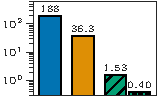
\includegraphics{figures/figure_10_a.pdf}
        \caption{SportsTables}
    \end{subfigure}%
    \begin{subfigure}[t]{.325\linewidth}
        \centering
        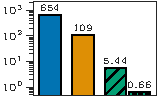
\includegraphics{figures/figure_10_b.pdf}
        \caption{Open Data}
    \end{subfigure}%
    \begin{subfigure}[t]{.325\linewidth}
        \centering
        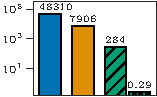
\includegraphics{figures/figure_10_c.pdf}
        \caption{GitTables}
    \end{subfigure}%
    \caption{Runtime comparison of \pscan, \binsort, and \approximate{} over 999 queries.}
    \Description{Bar chart showing runtime across all solutions and datasets.}
    \label{fig:runtime_comparison}
    % Figure width: 78.3722pt / 1.08in / 27mm
\end{figure}

\begin{figure}[t]
    \centering
    
\includegraphics{figures/figure_11_legend.pdf}\\
    \begin{subfigure}[t]{.03\linewidth}
        \centering
        
\includegraphics{figures/figure_11_label.pdf}
    \end{subfigure}%
    \hspace{-0.005\linewidth}%
    \begin{subfigure}[t]{.325\linewidth}
        \centering
        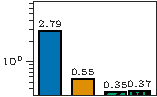
\includegraphics{figures/figure_11_a.pdf}
        \caption{SportsTables}
    \end{subfigure}%
    \begin{subfigure}[t]{.325\linewidth}
        \centering
        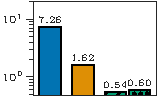
\includegraphics{figures/figure_11_b.pdf}
        \caption{Open Data}
    \end{subfigure}%
    \begin{subfigure}[t]{.325\linewidth}
        \centering
        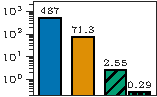
\includegraphics{figures/figure_11_c.pdf}
        \caption{GitTables}
    \end{subfigure}%
    \caption{Runtime comparison of \pscan, \binsort, and \approximate{} over 999 queries with low selectivity.}
    \Description{Bar chart showing runtime for low selectivity queries across all solutions and datasets.}
    \label{fig:runtime_comparison_low_selectivity}
    % Figure width: 78.3722pt / 1.08in / 27mm
\end{figure}

Figure~\ref{fig:runtime_comparison} shows an execution time comparison for our 999 test queries.
The figure highlights that \approximate{} is more than two orders of magnitude faster than \pscan and $20-28\times$ faster than \binsort on all three dataset collections.
Furthermore, we observe that \approximate{} achieves interactive execution times for each collection if we scale down the runtime to an individual predicate evaluation.

As we only benchmark the runtime of individual percentile predicates instead of large composite queries in this experiment, the result set $S$ can become quite large.
Therefore, we also ran a modified version of \system{} that performs all steps from Algorithm~\ref{alg:index_query} until line~\ref{alg:after_cluster} but returns a dummy result of size 1 to filter out the linear time impact of processing the result set.
This ``without results'' execution time demonstrates the potential runtime impact of $S$.
While the difference to the regular execution of \system{} is $4-5\times$ for SportsTables and Open Data, \system{} is another two orders of magnitude faster on GitTables when not returning results.
This shows how significant \system{}'s runtime advantage over the baselines is if the execution is not dominated by $S$ -- either because users run composite queries with multiple different predicates or because a percentile predicate itself has very low selectivity.

To specifically test the runtime of \system{} when a percentile predicate has very low selectivity, we simulated a restrictive column identifier that only matches 1\% of the histograms and then ran our benchmark queries on the resulting histogram subset.
The average selectivity of our queries when combining the column identifier and the distributional requirement lies at 0.5\%.
Figure~\ref{fig:runtime_comparison_low_selectivity} highlights that \system{} maintains its performance lead over the baselines for low-selectivity queries, while the relative advantage shrinks for the small dataset collections SportsTables and Open Data.
This is because \system{}'s runtime grows or shrinks logarithmically with the collection size while the baselines benefit linearly from a smaller collection.
We also see that the result set $S$ no longer impacts the runtime for the small collections.
Regarding GitTables, about $10\;000$ histograms remain after prefiltering so that \system{} still outperforms all baselines by orders of magnitude, consistent with Figure~\ref{fig:runtime_comparison}.
Overall, the experiment shows that \system{} is a superior choice in terms of runtime, especially for large-scale dataset search.

\paragraph{Scalability}
We investigate the scalability of \system{} by creating four versions of our largest collection GitTables, including each histogram 0.25, 0.5, 1, and 2 times on average to achieve a respective scaling factor.
Figure~\ref{fig:runtime_scalability} summarizes the runtime of \system{} for all scaling factors.
To account for the impact of the solution size $S$, we again conduct the experiment with and without processing the search results.
We see that the execution time of the runs that return results increases linearly with the scaling factor since $|S|$ also increases linearly with the scaling factor.
Contrarily, the runtime of \system{} is almost constant without returning results, highlighting its logarithmic scaling in the number of histograms and bins.

\paragraph{\approximate{}}

\begin{figure}[t]
    \centering
    \begin{minipage}[b]{0.47\linewidth}
        \centering
        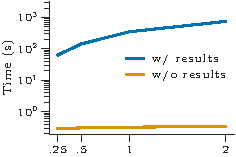
\includegraphics{figures/figure_12.pdf}
        \caption{Runtime on Git\-Tables across scaling factors.}
        \Description{Line chart showing runtime over scaling factor.}
        \label{fig:runtime_scalability}
        % Figure width: 113.33961pt / 1.568in / 39.8mm
    \end{minipage}%
    \hfill%
    \begin{minipage}[b]{0.49\linewidth}
        \centering
        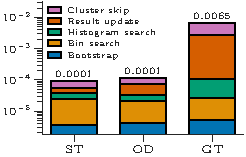
\includegraphics{figures/figure_13.pdf}
        \caption{Predicate evaluation runtime breakdown.}
        \Description{Stacked bar chart showing runtime of each \system{} phase over each dataset collection.}
        \label{fig:runtime_breakdown}
        % Figure width: 118.16359pt / 1.635in / 41.5mm
    \end{minipage}
\end{figure}

After reviewing the scalability of \system{}, we zoom into the individual phases of predicate evaluation with \approximate{}.
Due to the challenges of tracing a system-under-test without altering its performance~\cite{jain_art_1991}, we only measure the conceptually necessary steps of \system{} in this experiment.
Note that tracing those steps already increases a query's execution time by one order of magnitude due to logging overhead.

Figure~\ref{fig:runtime_breakdown} dissects the core operations of our index for the exemplary predicate $\cP_{*, 0.1, <, 50}$.
The experiment shows that the two most critical operations, bin and histogram search, scale sublinearly with the dataset collection size.
While bin search time is almost the same across collections, histogram search only grows by $7\times$ for GitTables, although the collection is $252\times$ and $73\times$ larger than the other two collections.
The result set update, on the other hand, scales linearly with $|S|$ and thus takes noticeably more time for GitTables.
Cluster skip partially also scales with $|S|$ as all histograms from a cluster might have to be added to $S$ depending on line~\ref{alg:cluster_skip} in Algorithm~\ref{alg:index_query}.

\paragraph{\exact{}}

\begin{figure}[t]
    \centering
    
\includegraphics{figures/figure_14_legend.pdf}\\
    \begin{subfigure}[t]{.03\linewidth}
        \centering
        
\includegraphics{figures/figure_14_label.pdf}
    \end{subfigure}%
    \hspace{-0.005\linewidth}%
    \begin{subfigure}[t]{.325\linewidth}
        \centering
        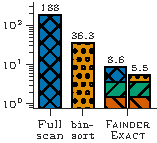
\includegraphics{figures/figure_14_a.pdf}
        \caption{SportsTables}
    \end{subfigure}%
    \begin{subfigure}[t]{.325\linewidth}
        \centering
        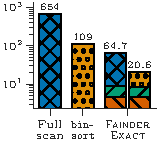
\includegraphics{figures/figure_14_b.pdf}
        \caption{Open Data}
    \end{subfigure}%
    \begin{subfigure}[t]{.325\linewidth}
        \centering
        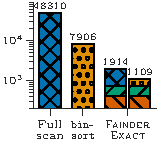
\includegraphics{figures/figure_14_c.pdf}
        \caption{GitTables}
    \end{subfigure}%
    \caption{Execution time breakdown of \exact{} compared to baselines for 999 queries.}
    \Description{Four bar charts showing the runtime of \pscan, \binsort, and \exact{} for each dataset collection.}
    \label{fig:exact_results}
\end{figure}

Building on the analysis of \approximate{}, we investigate the efficiency of our exact solution.
Figure~\ref{fig:exact_results} shows the runtime of its three phases compared to our exact baselines.
Since \pscan and \binsort both yield exact results, we can use either for the third stage of \exact{}.
Conceptually, \exact{} has no guaranteed speedup as the improvement depends on the combined pruning factor of the first two stages.
Nevertheless, in practice, it is $10-25\times$ faster than \pscan and $5-7\times$ faster than \binsort, as it can prune (a)~98\%, (b)~93\%, and (c)~98\% of the histograms on average for our benchmark queries.
Noticeably, the third iterative stage still dominates the runtime in many cases.\looseness=-1

Note that while \binsort appears like an overall better baseline, its performance depends not only on the number of histograms in a collection but also on the number of bins per histogram, as it creates an index entry for each bin.
However, we cannot control the number of bins per histogram in our setting since they are created by the data owners.
In a side experiment, we verified that the runtime of \binsort increases linearly if we simulate collections with more average bins per histogram.
Therefore, the optimal algorithm choice for stage three depends on the histogram collection, while both choices generally yield speedups over the baselines.

\paragraph{Index Construction}

\begin{figure}[t]
    \centering
    
\includegraphics{figures/figure_15_legend.pdf}\\
    \begin{subfigure}[t]{.03\linewidth}
        \centering
        
\includegraphics{figures/figure_15_label.pdf}
    \end{subfigure}%
    % \hspace{-0.6em}
    \begin{subfigure}[t]{.485\linewidth}
        \centering
        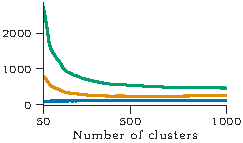
\includegraphics{figures/figure_15_a.pdf}
    \end{subfigure}%
    \begin{subfigure}[t]{.485\linewidth}
        \centering
        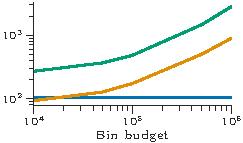
\includegraphics{figures/figure_15_b.pdf}
    \end{subfigure}%
    \caption{Construction time of \system{} on GitTables with a bin budget of $\boldsymbol{50\;000}$ (left) and 100 clusters (right).}
    \Description{Two line charts showing the runtime over the number of clusters (left) and the bin budget (right).}
    \label{fig:construction_time_gittables}
    % Figure width: 116.95668pt / 1.61in / 41.1mm
\end{figure}

In Figure~\ref{fig:construction_time_gittables}, we measure the index construction time on GitTables and vary the number of clusters $k$ while keeping the bin budget $\cB$ fixed and vice versa.
We divide index construction time into clustering and histogram alignment, separating rebinning and conversion for histogram alignment.
We observe that the impact of $k$ and $\cB$ on clustering time is negligible, as k-Means has robust scalability and \system{}'s aligned bins are only assigned after the histograms have been clustered.
Rebinning and conversion time decreases with an increasing $k$ because the index becomes smaller with more evenly distributed clusters, resulting in fewer percentiles to compute.
Conversely, $\cB$ increases histogram alignment time by increasing the number of percentiles in the index.
Overall, the index construction time for a reasonable selection of $k$ is feasible, considering that histogram insertion and deletion are incremental.
We only need to construct \system{} from scratch at the beginning or when processing significant bulk updates.


\subsection{Solution Effectiveness}
\label{sec:solution_effectiveness}

We analyze the effectiveness of \system{} in three parts:
We discuss a qualitative case study of distribution-aware dataset search on existing search engines, examine the findings of our hyperparameter grid search, and finally compare \system{}'s accuracy with our baselines.\looseness=-1

\paragraph{Case Study}
We conducted a qualitative case study to estimate the time a human needs to run a search with percentile requirements, combining keyword queries and manual investigation.
For this, we continued our initial motivating example to show the current user experience's shortcomings concretely.
We used Kaggle Datasets~\cite{kaggle_inc_kaggle_2024} in our study, as it is a comprehensive collection of datasets specifically intended for machine learning (i.e.,~a use case that benefits from percentile predicates).
As of February 2024, our example's keyword query ``lung cancer age'' yielded 67 results that our data scientist needs to review.
We make a conservative estimate and assume they need one minute per dataset on average, including datasets they can quickly rule out and datasets they have to download and analyze with a tool like Pandas.
This would take them about one hour instead of less than a second with \system{}.
Since users often search for datasets in a work context, this showcases the considerable economic potential of distribution-aware search.

\begin{figure*}[t]
    \setlength{\belowcaptionskip}{-4mm}
    \centering
    
\includegraphics{figures/figure_16_legend.pdf}\\
    \begin{subfigure}[t]{.03\linewidth}
        \centering
        
\includegraphics{figures/figure_16_label.pdf}
    \end{subfigure}%
    \hspace{-0.005\linewidth}%
    \begin{subfigure}[t]{.325\linewidth}
        \centering
        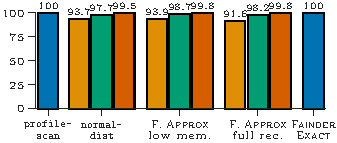
\includegraphics{figures/figure_16_a.pdf}
        \caption{SportsTables}
    \end{subfigure}%
    \begin{subfigure}[t]{.325\linewidth}
        \centering
        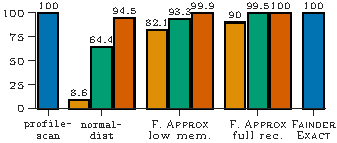
\includegraphics{figures/figure_16_b.pdf}
        \caption{Open Data}
    \end{subfigure}%
    \begin{subfigure}[t]{.325\linewidth}
        \centering
        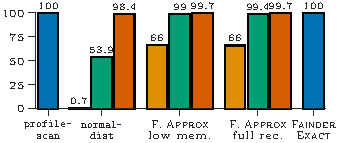
\includegraphics{figures/figure_16_c.pdf}
        \caption{GitTables}
    \end{subfigure}%
    \caption{$\boldsymbol{F_1}$ score of \pscan, \ndist, \approximate{}, and \exact{}, grouped by query selectivity.}
    \Description{Bar chart showing the $F_1$ score of each solution grouped by query selectivity and dataset collection.}
    \label{fig:accuracy_barchart_f1}
    % Figure width: 164.54433pt / 2.27in / 57.8mm
\end{figure*}

\paragraph{Hyperparameter Grid Search}
We conducted an extensive grid search on our validation query set to analyze \system{}'s configuration robustness.
Below, we summarize our key insights regarding the choice of clustering algorithm ($A$), clustering feature transformation ($T$), number of clusters ($k$), and bin budget ($\cB$).

($A$)
We examined three classes of clustering algorithms: density-based clustering with HDBSCAN~\cite{campello_density-based_2013}, agglomerative clustering, and k-Means.
Density-based clustering does not require choosing the hyperparameter $k$.
However, it can classify an arbitrarily large share of points as outliers.
This is detrimental in our setting since we need to index all histograms, and forming a heterogeneous outlier cluster yields catastrophic query accuracy within that cluster.
Agglomerative clustering makes no assumptions about the feature distribution and is robust to outliers.
Yet, it does not achieve a feasible runtime for large dataset collections; we aborted a grid search on GitTables because it took more than 2.5 days, while k-Means took less than 5 hours for the same search.
k-Means achieved the best overall performance, producing clusterings that yield accurate indices within less than two minutes for each dataset collection.

($T$)
Next to a quantile transform~\cite{pedregosa_scikit-learn_2011}, we also investigated simple and robust standardization, as well as no feature preprocessing in our experiments.
If the features fall into clearly separable clusters by default, such as with SportsTables, we found that simple standardization or no preprocessing can yield the best results.
However, across dataset collections and index configurations, the quantile transform is most robust to heterogeneous histogram features and thus produces the smallest and most accurate indices on average.

($k$)
Using a reasonably large value for $k$ (> 100) generally yields a good result accuracy.
Increasing $k$ beyond this point presents a trade-off between index size and runtime, as $k$ has a linear impact on the runtime but reduces the number of computed percentiles.

($\cB$)
The bin budget should be chosen according to the memory capacity and in conjunction with $k$, as more clusters result in smaller indices.
A higher bin budget generally produces more precise indices, although with diminishing returns.

Based on our grid search results, we selected index configurations that optimize result accuracy and reduce the index size for our other experiments.
Concretely, we use k-Means and preprocess all collections but SportsTables using a quantile transform.
In addition, we use (230, 250, 750) clusters and (5K, 50K, 100K) bins for SportsTables, Open Data, and GitTables.

\paragraph{Accuracy Comparison}
Figure~\ref{fig:accuracy_barchart_f1} presents the $F_1$ score of \pscan, \ndist, \approximate{} low memory (based on rebinning), \approximate{} full recall (based on conversion), as well as \exact{}.
For the approximate solutions, we group the results by query selectivity.
We observe that all approaches perform best on SportsTables, with its manually curated datasets that often match a normal distribution.
For Open Data and GitTables, the results are more diverse.
\ndist performs consistently worse than \approximate{} variants, especially on the more challenging collections.
\approximate{} constructed with conversion performs better than rebinning on Open Data due to its guaranteed recall of 1 but at the cost of using more memory.
Overall, low and medium selectivity queries have a lower $F_1$ score.

\begin{figure}[t]
    \setlength{\belowcaptionskip}{-1mm}
    \centering
    
\includegraphics{figures/figure_17_legend.pdf}\\
    \begin{subfigure}[t]{.49\linewidth}
        \centering
        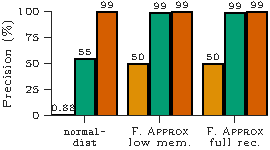
\includegraphics[scale=0.91]{figures/figure_17_a.pdf}
    \end{subfigure}%
    \hfill%
    \begin{subfigure}[t]{.49\linewidth}
        \centering
        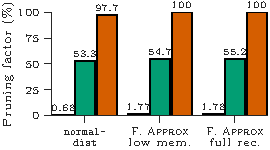
\includegraphics[scale=0.91]{figures/figure_17_b.pdf}
    \end{subfigure}%
    \caption{Precision and pruning factor of approximate solutions on GitTables.}
    \Description{Two bar charts showing the precision (left) and pruning factor (right) of the approximate solutions on GitTables, grouped by query selectivity.}
    \label{fig:accuracy_barchart_approx}
    % Figure width: 118.16359pt / 1.63in / 41.5mm
\end{figure}

To explain the worse $F_1$ score for queries with lower selectivity, we show the precision and pruning factor of approximate solutions on GitTables in Figure~\ref{fig:accuracy_barchart_approx}.
Comparing the results to the $F_1$ score from Figure~\ref{fig:accuracy_barchart_f1}~(c), we observe that a lower precision predominantly causes the performance decrease.
Considering the pruning factor, we see that \approximate{} variants nevertheless filter out around 98\% of the histograms.
If the cardinality of the true result is low, a small absolute number of false positives can cause a sizeable relative performance decrease in precision.
Thus, we argue that the worse performance for low selectivity queries has limited practical impact, as the absolute number of false results is small.

\begin{figure}[t]
    \setlength{\belowcaptionskip}{-2mm}
    \centering
    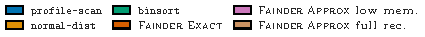
\includegraphics{figures/figure_18_legend.pdf}\\
    \begin{subfigure}[t]{.03\linewidth}
        \centering
        
\includegraphics{figures/figure_18_label.pdf}
    \end{subfigure}%
    \hspace{-0.005\linewidth}%
    \begin{subfigure}[t]{.325\linewidth}
        \centering
        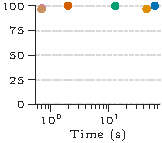
\includegraphics{figures/figure_18_a.pdf}
        \caption{SportsTables}
    \end{subfigure}%
    \begin{subfigure}[t]{.325\linewidth}
        \centering
        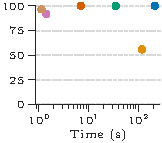
\includegraphics{figures/figure_18_b.pdf}
        \caption{Open Data}
    \end{subfigure}%
    \begin{subfigure}[t]{.325\linewidth}
        \centering
        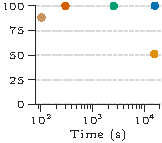
\includegraphics{figures/figure_18_c.pdf}
        \caption{GitTables}
    \end{subfigure}%
    \caption{$\boldsymbol{F_1}$ score over runtime of \pscan, \ndist, \binsort, and \system{} variants.}
    \Description{Three scatter plots showing the $F_1$ score over the runtime of all solutions across the three dataset collections.}
    \label{fig:accuracy_scatterplot_f1}
\end{figure}

We also jointly investigated each approach's result accuracy and runtime performance.
Figure~\ref{fig:accuracy_scatterplot_f1} highlights that \system{} strictly dominates the baselines in a skyline analysis for all three dataset collections.
\exact{} achieves 100\% $F_1$ score in $5-53\times$ less time than the exact baselines.
\approximate{} variants achieve the fastest runtime overall at the cost of producing a few false results.
\ndist presents a worse accuracy-runtime trade-off than our solutions on all collections.
Therefore, we argue that its space savings ($O(2)$ vs. $O(\cB_c)$ per column) are not justified unless the vast majority of columns follow a normal distribution.


\subsection{Micro-Benchmarks}
\label{sec:micro_benchmarks}

We conclude our experimental evaluation with a holistic analysis of the impact of the number of clusters and the bin budget on all three dimensions of \system{}'s performance.
Finally, we distill our investigation into two easy-to-follow steps for practitioners.

\paragraph{Impact of Clustering}

\begin{figure}[t]
    \centering
    \includegraphics[scale=0.965]{figures/figure_19.pdf}
    \caption{Query runtime, index size, and $\boldsymbol{F_1}$ score of \approximate{} over the number of clusters on Open Data.}
    \Description{Line chart with three y-axes showing the runtime, index size, and $F_1$ score of \system{} over the number of clusters on Open Data.}
    \label{fig:microbenchmark_open_data_k}
    % Figure width: 241.14749pt / 3.33in / 84.7mm
\end{figure}

Figure~\ref{fig:microbenchmark_open_data_k} demonstrates the interplay of runtime, result accuracy, and index size for a varying number of clusters and $50\;000$ bins on Open Data.
Without a sufficient number of clusters ($k<10$ in this case), accuracy and index size deteriorate significantly as the aligned bins become less precise and the clusters less balanced.
For $k=1$, the memory consumption (and index construction time) becomes unfeasible.
Thus, clustering is a critical component of \system{}.
Fortunately, the choice of $k$ for larger values is robust concerning the result accuracy, making \system{} easy to configure.
This experiment supports our grid search's finding that increasing $k$ presents a trade-off between index size and runtime.
However, when comparing the two blue lines, we see that the runtime impact of a growing $k$ is partly mitigated if we also consider the result processing time.
This is because more clusters can yield a more precise index, resulting in a smaller result set size.\looseness=-1


\paragraph{Impact of Bin Budget}

\begin{figure}[t]
    \centering
    \includegraphics[scale=0.965]{figures/figure_20.pdf}
    \caption{Query runtime, index size, and $\boldsymbol{F_1}$ score of \approximate{} over varying bin budgets on Open Data.}
    \Description{Line chart with three y-axes showing the runtime, index size, and $F_1$ score of \system{} over the bin budget on Open Data.}
    \label{fig:microbenchmark_open_data_b}
\end{figure}

In Figure~\ref{fig:microbenchmark_open_data_b}, we fix the number of clusters to 100 and vary the bin budget.
We observe that (1) the runtime is robust to the bin budget due to our use of binary search; (2) the $F_1$ score increases from 84\% to 93\% and 96\% with an increasing bin budget, although at diminishing returns; and (3) the index size grows linearly with $\cB$.
Note that, in general, the size of \system{} scales with the number but not the size of the datasets.
This makes \system{} relatively large for dataset collections with many small datasets, such as GitTables.
On the other side, it is robust to dataset collections for machine learning, where individual datasets can take up many gigabytes or even terabytes of storage.

\paragraph{Practical Guidance for Index Configuration}
First, select the largest possible value of $k$ acceptable for runtime.
To ensure performance, $k$ should be at least $100\times$ smaller than $|\cH|$.
Then, choose the largest possible value of $\cB$ acceptable in terms of index size.

%!TEX root = ../main.tex

\section{Related Work}
\label{sec:related_work}

Prior work on dataset search can be broadly classified into data lake navigation~\cite{nargesian_data_2023, nargesian_organizing_2020, ouellette_ronin_2021}, data discovery by example~\cite{rezig_dice_2021}, task-driven search~\cite{galhotra_metam_2023} for machine learning pipelines~\cite{behme_art_2023}, and query-driven search.
We focus our discussion on the latter, as the other three concepts require access to a dataset collection's raw data.
Within query-driven dataset search, we distinguish two central settings: data lakes, where the raw data are fully accessible, and metadata-based search, where search engines must rely on data owner-provided, heterogeneous, and potentially missing metadata.
Moreover, there are different types of search predicates.
In the following, we specifically discuss dis\-tri\-bu\-tion-aware and keyword search.
We close by reviewing related work on data profiling and histograms.\looseness=-1

\paragraph{Full Data Access}
There is a long line of prior work on data discovery in data lakes~\cite{bharadwaj_discovering_2021, bogatu_dataset_2020, castro_fernandez_aurum_2018, esmailoghli_mate_2022, gong_ver_2023, koutras_valentine_2021, miller_making_2018, zhang_dsdd_2021, zhang_finding_2020, gong_nexus_2024}.
However, data lake-focused discovery techniques assume full data access and thus are not applicable in our problem setting.

\paragraph{Metadata Access}
Existing metadata-based dataset search engines, such as Google Dataset Search~\cite{noy_google_2019} and CKAN~\cite{open_knowledge_foundation_ckan_2022}, are limited to keyword search (possibly extended with facets).
Auctus~\cite{castelo_auctus_2021} is a hybrid between the full and metadata access settings, as it collects existing metadata from multiple federated data repositories but also downloads raw data from openly available datasets to profile them individually.
Based on this auxiliary information, Auctus allows users to add advanced facets to their queries, such as spatiotemporal or column type filters.
In general, dataset search on metadata has not yet been explored as thoroughly as data lake search.
The continuum between the two settings, where more or less metadata and samples from a dataset are available, is an exciting direction for future work.
In practice, solutions must deal with varying degrees of dataset profile heterogeneity and information granularity.

\paragraph{Distribution-Aware Search}
Recently, \textcite{asudeh_towards_2022} developed a system vision for the new field of distribution-aware data discovery.
While their vision targets the data lake setting, it highlights the importance of distributional queries over dataset collections.
For the same setting, \textcite{nargesian_tailoring_2021} proposed distribution tailoring to meet fairness requirements in data integration and \textcite{chai_selective_2022} presented distribution-aware data augmentation for model training.
Our work expands distribution-aware dataset search and proposes solutions that do not require raw data access.

\paragraph{Keyword Search}
The extensive work on keyword search is surveyed in~\cite{le_survey_2016, park_keyword_2011, yang_keyword_2021, yu_keyword_2010}.
Our contributions complement keyword search, as our query model incorporates keyword predicates and integrates them with distribution-aware (i.e.,~percentile) predicates.
Recent advances in large language models have led to a new line of work focusing on retrieving relevant datasets given a natural language query~\cite{herzig_open_2021, wang_retrieving_2021, wang_solo_2023}.
However, these works either focus on textual information about datasets or require full data access, whereas we target distribution-aware queries on heterogeneous synopses.\looseness=-1

\paragraph{Data Profiling}
Prior work on data profiling~\cite{abedjan_profiling_2015} and cleaning~\cite{abedjan_detecting_2016, halevy_goods_2016, galhotra_dataprism_2022} is orthogonal to our contributions on searching over heterogeneous histograms.
There are various methods for creating histograms~\cite{cormode_synopses_2011}, such as equi-height or equi-width, but the problem of optimizing histograms to reduce estimation error~\cite{behar_optimal_2020, jagadish_optimal_1998} or improve visibility is complementary to our setting, where data owners generate histograms independently of the search engine.

%!TEX root = ../main.tex

\section{Conclusion and Future Work}
\label{sec:conclusion}

We introduced the novel problem of distribution-aware dataset search on decentralized data repositories and proposed \system{}, a fast and accurate index for percentile predicates.
\system{} offers exact and approximate solutions, achieving more than two orders of magnitude speedups over baseline approaches and dominating the start-of-the-art in an accuracy-runtime skyline analysis.

Our work gives rise to several interesting directions for future work, of which we discuss three that we consider most important.
To effectively integrate \system{} into a system, a search engine should combine it with semantic keyword similarity search and dataset profile alignment techniques to amplify the column identifier in a percentile predicate.
Once a dataset search engine supports multiple predicate types, query planning and optimization are paramount problems.
Beyond system integration, we see an opportunity to leverage our query model for designing distribution-aware dataset search predicates based on data synopses other than histograms, such as sketches.
For example, using synopses to rank each dataset's similarity to an input dataset or a reference distribution is challenging.
Lastly, while \system{} can approximate percentile predicates with two-sided ranges via a combination of one-sided predicates, developing an index that natively supports range predicates presents novel research challenges.

\begin{acks}
    We gratefully acknowledge funding from the German Federal Ministry of Education and Research under the grants BIFOLD24B and 01IS17052 (for the Software Campus project FDaaS).
\end{acks}

\flushcolsend


\printbibliography

\end{document}
\endinput
